
%% bare_jrnl_compsoc.tex
%% V1.3
%% 2007/01/11
%% by Michael Shell
%% See:
%% http://www.michaelshell.org/
%% for current contact information.
%%
%% This is a skeleton file demonstrating the use of IEEEtran.cls
%% (requires IEEEtran.cls version 1.7 or later) with an IEEE Computer
%% Society journal paper.
%%
%% Support sites:
%% http://www.michaelshell.org/tex/ieeetran/
%% http://www.ctan.org/tex-archive/macros/latex/contrib/IEEEtran/
%% and
%% http://www.ieee.org/

%%*************************************************************************
%% Legal Notice:
%% This code is offered as-is without any warranty either expressed or
%% implied; without even the implied warranty of MERCHANTABILITY or
%% FITNESS FOR A PARTICULAR PURPOSE!
%% User assumes all risk.
%% In no event shall IEEE or any contributor to this code be liable for
%% any damages or losses, including, but not limited to, incidental,
%% consequential, or any other damages, resulting from the use or misuse
%% of any information contained here.
%%
%% All comments are the opinions of their respective authors and are not
%% necessarily endorsed by the IEEE.
%%
%% This work is distributed under the LaTeX Project Public License (LPPL)
%% ( http://www.latex-project.org/ ) version 1.3, and may be freely used,
%% distributed and modified. A copy of the LPPL, version 1.3, is included
%% in the base LaTeX documentation of all distributions of LaTeX released
%% 2003/12/01 or later.
%% Retain all contribution notices and credits.
%% ** Modified files should be clearly indicated as such, including  **
%% ** renaming them and changing author support contact information. **
%%
%% File list of work: IEEEtran.cls, IEEEtran_HOWTO.pdf, bare_adv.tex,
%%                    bare_conf.tex, bare_jrnl.tex, bare_jrnl_compsoc.tex
%%*************************************************************************

% *** Authors should verify (and, if needed, correct) their LaTeX system  ***
% *** with the testflow diagnostic prior to trusting their LaTeX platform ***
% *** with production work. IEEE's font choices can trigger bugs that do  ***
% *** not appear when using other class files.                            ***
% The testflow support page is at:
% http://www.michaelshell.org/tex/testflow/




% Note that the a4paper option is mainly intended so that authors in
% countries using A4 can easily print to A4 and see how their papers will
% look in print - the typesetting of the document will not typically be
% affected with changes in paper size (but the bottom and side margins will).
% Use the testflow package mentioned above to verify correct handling of
% both paper sizes by the user's LaTeX system.
%
% Also note that the "draftcls" or "draftclsnofoot", not "draft", option
% should be used if it is desired that the figures are to be displayed in
% draft mode.
%
% The Computer Society usually requires 10pt for submissions.
%

\documentclass[10pt,journal,cspaper,compsoc]{IEEEtran}
\usepackage{graphicx}
\usepackage{amsthm}
\usepackage{algpseudocode}
\usepackage{algorithm}
\usepackage{amsmath}

\algrenewcommand{\algorithmicrequire}{\textbf{Input:}}
\algrenewcommand{\algorithmicensure}{\textbf{Output:}}
\renewcommand{\algorithmicforall}{\textbf{for each}}
%
% If IEEEtran.cls has not been installed into the LaTeX system files,
% manually specify the path to it like:
% \documentclass[12pt,journal,compsoc]{../sty/IEEEtran}





% Some very useful LaTeX packages include:
% (uncomment the ones you want to load)


% *** MISC UTILITY PACKAGES ***
%
%\usepackage{ifpdf}
% Heiko Oberdiek's ifpdf.sty is very useful if you need conditional
% compilation based on whether the output is pdf or dvi.
% usage:
% \ifpdf
%   % pdf code
% \else
%   % dvi code
% \fi
% The latest version of ifpdf.sty can be obtained from:
% http://www.ctan.org/tex-archive/macros/latex/contrib/oberdiek/
% Also, note that IEEEtran.cls V1.7 and later provides a builtin
% \ifCLASSINFOpdf conditional that works the same way.
% When switching from latex to pdflatex and vice-versa, the compiler may
% have to be run twice to clear warning/error messages.






% *** CITATION PACKAGES ***
%
\ifCLASSOPTIONcompsoc
  % IEEE Computer Society needs nocompress option
  % requires cite.sty v4.0 or later (November 2003)
  % \usepackage[nocompress]{cite}
\else
  % normal IEEE
  % \usepackage{cite}
\fi
% cite.sty was written by Donald Arseneau
% V1.6 and later of IEEEtran pre-defines the format of the cite.sty package
% \cite{} output to follow that of IEEE. Loading the cite package will
% result in citation numbers being automatically sorted and properly
% "compressed/ranged". e.g., [1], [9], [2], [7], [5], [6] without using
% cite.sty will become [1], [2], [5]--[7], [9] using cite.sty. cite.sty's
% \cite will automatically add leading space, if needed. Use cite.sty's
% noadjust option (cite.sty V3.8 and later) if you want to turn this off.
% cite.sty is already installed on most LaTeX systems. Be sure and use
% version 4.0 (2003-05-27) and later if using hyperref.sty. cite.sty does
% not currently provide for hyperlinked citations.
% The latest version can be obtained at:
% http://www.ctan.org/tex-archive/macros/latex/contrib/cite/
% The documentation is contained in the cite.sty file itself.
%
% Note that some packages require special options to format as the Computer
% Society requires. In particular, Computer Society  papers do not use
% compressed citation ranges as is done in typical IEEE papers
% (e.g., [1]-[4]). Instead, they list every citation separately in order
% (e.g., [1], [2], [3], [4]). To get the latter we need to load the cite
% package with the nocompress option which is supported by cite.sty v4.0
% and later. Note also the use of a CLASSOPTION conditional provided by
% IEEEtran.cls V1.7 and later.





% *** GRAPHICS RELATED PACKAGES ***
%
\ifCLASSINFOpdf
  % \usepackage[pdftex]{graphicx}
  % declare the path(s) where your graphic files are
  % \graphicspath{{../pdf/}{../jpeg/}}
  % and their extensions so you won't have to specify these with
  % every instance of \includegraphics
  % \DeclareGraphicsExtensions{.pdf,.jpeg,.png}
\else
  % or other class option (dvipsone, dvipdf, if not using dvips). graphicx
  % will default to the driver specified in the system graphics.cfg if no
  % driver is specified.
  % \usepackage[dvips]{graphicx}
  % declare the path(s) where your graphic files are
  % \graphicspath{{../eps/}}
  % and their extensions so you won't have to specify these with
  % every instance of \includegraphics
  % \DeclareGraphicsExtensions{.eps}
\fi
% graphicx was written by David Carlisle and Sebastian Rahtz. It is
% required if you want graphics, photos, etc. graphicx.sty is already
% installed on most LaTeX systems. The latest version and documentation can
% be obtained at:
% http://www.ctan.org/tex-archive/macros/latex/required/graphics/
% Another good source of documentation is "Using Imported Graphics in
% LaTeX2e" by Keith Reckdahl which can be found as epslatex.ps or
% epslatex.pdf at: http://www.ctan.org/tex-archive/info/
%
% latex, and pdflatex in dvi mode, support graphics in encapsulated
% postscript (.eps) format. pdflatex in pdf mode supports graphics
% in .pdf, .jpeg, .png and .mps (metapost) formats. Users should ensure
% that all non-photo figures use a vector format (.eps, .pdf, .mps) and
% not a bitmapped formats (.jpeg, .png). IEEE frowns on bitmapped formats
% which can result in "jaggedy"/blurry rendering of lines and letters as
% well as large increases in file sizes.
%
% You can find documentation about the pdfTeX application at:
% http://www.tug.org/applications/pdftex





% *** MATH PACKAGES ***
%
%\usepackage[cmex10]{amsmath}
% A popular package from the American Mathematical Society that provides
% many useful and powerful commands for dealing with mathematics. If using
% it, be sure to load this package with the cmex10 option to ensure that
% only type 1 fonts will utilized at all point sizes. Without this option,
% it is possible that some math symbols, particularly those within
% footnotes, will be rendered in bitmap form which will result in a
% document that can not be IEEE Xplore compliant!
%
% Also, note that the amsmath package sets \interdisplaylinepenalty to 10000
% thus preventing page breaks from occurring within multiline equations. Use:
%\interdisplaylinepenalty=2500
% after loading amsmath to restore such page breaks as IEEEtran.cls normally
% does. amsmath.sty is already installed on most LaTeX systems. The latest
% version and documentation can be obtained at:
% http://www.ctan.org/tex-archive/macros/latex/required/amslatex/math/





% *** SPECIALIZED LIST PACKAGES ***
%
%\usepackage{algorithmic}
% algorithmic.sty was written by Peter Williams and Rogerio Brito.
% This package provides an algorithmic environment fo describing algorithms.
% You can use the algorithmic environment in-text or within a figure
% environment to provide for a floating algorithm. Do NOT use the algorithm
% floating environment provided by algorithm.sty (by the same authors) or
% algorithm2e.sty (by Christophe Fiorio) as IEEE does not use dedicated
% algorithm float types and packages that provide these will not provide
% correct IEEE style captions. The latest version and documentation of
% algorithmic.sty can be obtained at:
% http://www.ctan.org/tex-archive/macros/latex/contrib/algorithms/
% There is also a support site at:
% http://algorithms.berlios.de/index.html
% Also of interest may be the (relatively newer and more customizable)
% algorithmicx.sty package by Szasz Janos:
% http://www.ctan.org/tex-archive/macros/latex/contrib/algorithmicx/




% *** ALIGNMENT PACKAGES ***
%
%\usepackage{array}
% Frank Mittelbach's and David Carlisle's array.sty patches and improves
% the standard LaTeX2e array and tabular environments to provide better
% appearance and additional user controls. As the default LaTeX2e table
% generation code is lacking to the point of almost being broken with
% respect to the quality of the end results, all users are strongly
% advised to use an enhanced (at the very least that provided by array.sty)
% set of table tools. array.sty is already installed on most systems. The
% latest version and documentation can be obtained at:
% http://www.ctan.org/tex-archive/macros/latex/required/tools/


%\usepackage{mdwmath}
%\usepackage{mdwtab}
% Also highly recommended is Mark Wooding's extremely powerful MDW tools,
% especially mdwmath.sty and mdwtab.sty which are used to format equations
% and tables, respectively. The MDWtools set is already installed on most
% LaTeX systems. The lastest version and documentation is available at:
% http://www.ctan.org/tex-archive/macros/latex/contrib/mdwtools/


% IEEEtran contains the IEEEeqnarray family of commands that can be used to
% generate multiline equations as well as matrices, tables, etc., of high
% quality.


%\usepackage{eqparbox}
% Also of notable interest is Scott Pakin's eqparbox package for creating
% (automatically sized) equal width boxes - aka "natural width parboxes".
% Available at:
% http://www.ctan.org/tex-archive/macros/latex/contrib/eqparbox/





% *** SUBFIGURE PACKAGES ***
%\ifCLASSOPTIONcompsoc
%\usepackage[tight,normalsize,sf,SF]{subfigure}
%\else
%\usepackage[tight,footnotesize]{subfigure}
%\fi
% subfigure.sty was written by Steven Douglas Cochran. This package makes it
% easy to put subfigures in your figures. e.g., "Figure 1a and 1b". For IEEE
% work, it is a good idea to load it with the tight package option to reduce
% the amount of white space around the subfigures. Computer Society papers
% use a larger font and \sffamily font for their captions, hence the
% additional options needed under compsoc mode. subfigure.sty is already
% installed on most LaTeX systems. The latest version and documentation can
% be obtained at:
% http://www.ctan.org/tex-archive/obsolete/macros/latex/contrib/subfigure/
% subfigure.sty has been superceeded by subfig.sty.


%\ifCLASSOPTIONcompsoc
%  \usepackage[caption=false]{caption}
%  \usepackage[font=normalsize,labelfont=sf,textfont=sf]{subfig}
%\else
%  \usepackage[caption=false]{caption}
%  \usepackage[font=footnotesize]{subfig}
%\fi
% subfig.sty, also written by Steven Douglas Cochran, is the modern
% replacement for subfigure.sty. However, subfig.sty requires and
% automatically loads Axel Sommerfeldt's caption.sty which will override
% IEEEtran.cls handling of captions and this will result in nonIEEE style
% figure/table captions. To prevent this problem, be sure and preload
% caption.sty with its "caption=false" package option. This is will preserve
% IEEEtran.cls handing of captions. Version 1.3 (2005/06/28) and later
% (recommended due to many improvements over 1.2) of subfig.sty supports
% the caption=false option directly:
%\ifCLASSOPTIONcompsoc
%  \usepackage[caption=false,font=normalsize,labelfont=sf,textfont=sf]{subfig}
%\else
%  \usepackage[caption=false,font=footnotesize]{subfig}
%\fi
%
% The latest version and documentation can be obtained at:
% http://www.ctan.org/tex-archive/macros/latex/contrib/subfig/
% The latest version and documentation of caption.sty can be obtained at:
% http://www.ctan.org/tex-archive/macros/latex/contrib/caption/




% *** FLOAT PACKAGES ***
%
%\usepackage{fixltx2e}
% fixltx2e, the successor to the earlier fix2col.sty, was written by
% Frank Mittelbach and David Carlisle. This package corrects a few problems
% in the LaTeX2e kernel, the most notable of which is that in current
% LaTeX2e releases, the ordering of single and double column floats is not
% guaranteed to be preserved. Thus, an unpatched LaTeX2e can allow a
% single column figure to be placed prior to an earlier double column
% figure. The latest version and documentation can be found at:
% http://www.ctan.org/tex-archive/macros/latex/base/



%\usepackage{stfloats}
% stfloats.sty was written by Sigitas Tolusis. This package gives LaTeX2e
% the ability to do double column floats at the bottom of the page as well
% as the top. (e.g., "\begin{figure*}[!b]" is not normally possible in
% LaTeX2e). It also provides a command:
%\fnbelowfloat
% to enable the placement of footnotes below bottom floats (the standard
% LaTeX2e kernel puts them above bottom floats). This is an invasive package
% which rewrites many portions of the LaTeX2e float routines. It may not work
% with other packages that modify the LaTeX2e float routines. The latest
% version and documentation can be obtained at:
% http://www.ctan.org/tex-archive/macros/latex/contrib/sttools/
% Documentation is contained in the stfloats.sty comments as well as in the
% presfull.pdf file. Do not use the stfloats baselinefloat ability as IEEE
% does not allow \baselineskip to stretch. Authors submitting work to the
% IEEE should note that IEEE rarely uses double column equations and
% that authors should try to avoid such use. Do not be tempted to use the
% cuted.sty or midfloat.sty packages (also by Sigitas Tolusis) as IEEE does
% not format its papers in such ways.




%\ifCLASSOPTIONcaptionsoff
%  \usepackage[nomarkers]{endfloat}
% \let\MYoriglatexcaption\caption
% \renewcommand{\caption}[2][\relax]{\MYoriglatexcaption[#2]{#2}}
%\fi
% endfloat.sty was written by James Darrell McCauley and Jeff Goldberg.
% This package may be useful when used in conjunction with IEEEtran.cls'
% captionsoff option. Some IEEE journals/societies require that submissions
% have lists of figures/tables at the end of the paper and that
% figures/tables without any captions are placed on a page by themselves at
% the end of the document. If needed, the draftcls IEEEtran class option or
% \CLASSINPUTbaselinestretch interface can be used to increase the line
% spacing as well. Be sure and use the nomarkers option of endfloat to
% prevent endfloat from "marking" where the figures would have been placed
% in the text. The two hack lines of code above are a slight modification of
% that suggested by in the endfloat docs (section 8.3.1) to ensure that
% the full captions always appear in the list of figures/tables - even if
% the user used the short optional argument of \caption[]{}.
% IEEE papers do not typically make use of \caption[]'s optional argument,
% so this should not be an issue. A similar trick can be used to disable
% captions of packages such as subfig.sty that lack options to turn off
% the subcaptions:
% For subfig.sty:
% \let\MYorigsubfloat\subfloat
% \renewcommand{\subfloat}[2][\relax]{\MYorigsubfloat[]{#2}}
% For subfigure.sty:
% \let\MYorigsubfigure\subfigure
% \renewcommand{\subfigure}[2][\relax]{\MYorigsubfigure[]{#2}}
% However, the above trick will not work if both optional arguments of
% the \subfloat/subfig command are used. Furthermore, there needs to be a
% description of each subfigure *somewhere* and endfloat does not add
% subfigure captions to its list of figures. Thus, the best approach is to
% avoid the use of subfigure captions (many IEEE journals avoid them anyway)
% and instead reference/explain all the subfigures within the main caption.
% The latest version of endfloat.sty and its documentation can obtained at:
% http://www.ctan.org/tex-archive/macros/latex/contrib/endfloat/
%
% The IEEEtran \ifCLASSOPTIONcaptionsoff conditional can also be used
% later in the document, say, to conditionally put the References on a
% page by themselves.




% *** PDF, URL AND HYPERLINK PACKAGES ***
%
%\usepackage{url}
% url.sty was written by Donald Arseneau. It provides better support for
% handling and breaking URLs. url.sty is already installed on most LaTeX
% systems. The latest version can be obtained at:
% http://www.ctan.org/tex-archive/macros/latex/contrib/misc/
% Read the url.sty source comments for usage information. Basically,
% \url{my_url_here}.





% *** Do not adjust lengths that control margins, column widths, etc. ***
% *** Do not use packages that alter fonts (such as pslatex).         ***
% There should be no need to do such things with IEEEtran.cls V1.6 and later.
% (Unless specifically asked to do so by the journal or conference you plan
% to submit to, of course. )


% correct bad hyphenation here
\hyphenation{op-tical net-works semi-conduc-tor}


\begin{document}
%
% paper title
% can use linebreaks \\ within to get better formatting as desired
\title{Efficiently Identify the failure-inducing schemas}
%
%
% author names and IEEE memberships
% note positions of commas and nonbreaking spaces ( ~ ) LaTeX will not break
% a structure at a ~ so this keeps an author's name from being broken across
% two lines.
% use \thanks{} to gain access to the first footnote area
% a separate \thanks must be used for each paragraph as LaTeX2e's \thanks
% was not built to handle multiple paragraphs
%
%
%\IEEEcompsocitemizethanks is a special \thanks that produces the bulleted
% lists the Computer Society journals use for "first footnote" author
% affiliations. Use \IEEEcompsocthanksitem which works much like \item
% for each affiliation group. When not in compsoc mode,
% \IEEEcompsocitemizethanks becomes like \thanks and
% \IEEEcompsocthanksitem becomes a line break with idention. This
% facilitates dual compilation, although admittedly the differences in the
% desired content of \author between the different types of papers makes a
% one-size-fits-all approach a daunting prospect. For instance, compsoc
% journal papers have the author affiliations above the "Manuscript
% received ..."  text while in non-compsoc journals this is reversed. Sigh.

\author{Xintao~Niu,~
        Changhai~Nie,~\IEEEmembership{Member,~IEEE,}
        and~~% <-this % stops a space
\IEEEcompsocitemizethanks{\IEEEcompsocthanksitem M. Shell is with the Department
of Electrical and Computer Engineering, Georgia Institute of Technology, Atlanta,
GA, 30332.\protect\\
% note need leading \protect in front of \\ to get a newline within \thanks as
% \\ is fragile and will error, could use \hfil\break instead.
E-mail: see http://www.michaelshell.org/contact.html
\IEEEcompsocthanksitem J. Doe and J. Doe are with Anonymous University.}% <-this % stops a space
\thanks{}}

% note the % following the last \IEEEmembership and also \thanks -
% these prevent an unwanted space from occurring between the last author name
% and the end of the author line. i.e., if you had this:
%
% \author{....lastname \thanks{...} \thanks{...} }
%                     ^------------^------------^----Do not want these spaces!
%
% a space would be appended to the last name and could cause every name on that
% line to be shifted left slightly. This is one of those "LaTeX things". For
% instance, "\textbf{A} \textbf{B}" will typeset as "A B" not "AB". To get
% "AB" then you have to do: "\textbf{A}\textbf{B}"
% \thanks is no different in this regard, so shield the last } of each \thanks
% that ends a line with a % and do not let a space in before the next \thanks.
% Spaces after \IEEEmembership other than the last one are OK (and needed) as
% you are supposed to have spaces between the names. For what it is worth,
% this is a minor point as most people would not even notice if the said evil
% space somehow managed to creep in.



% The paper headers
\markboth{Journal of \LaTeX\ Class Files,~Vol.~6, No.~1, January~2007}%
{Shell \MakeLowercase{\textit{et al.}}: Bare Demo of IEEEtran.cls for Computer Society Journals}
% The only time the second header will appear is for the odd numbered pages
% after the title page when using the twoside option.
%
% *** Note that you probably will NOT want to include the author's ***
% *** name in the headers of peer review papers.                   ***
% You can use \ifCLASSOPTIONpeerreview for conditional compilation here if
% you desire.



% The publisher's ID mark at the bottom of the page is less important with
% Computer Society journal papers as those publications place the marks
% outside of the main text columns and, therefore, unlike regular IEEE
% journals, the available text space is not reduced by their presence.
% If you want to put a publisher's ID mark on the page you can do it like
% this:
%\IEEEpubid{0000--0000/00\$00.00~\copyright~2007 IEEE}
% or like this to get the Computer Society new two part style.
%\IEEEpubid{\makebox[\columnwidth]{\hfill 0000--0000/00/\$00.00~\copyright~2007 IEEE}%
%\hspace{\columnsep}\makebox[\columnwidth]{Published by the IEEE Computer Society\hfill}}
% Remember, if you use this you must call \IEEEpubidadjcol in the second
% column for its text to clear the IEEEpubid mark (Computer Society jorunal
% papers don't need this extra clearance.)




% for Computer Society papers, we must declare the abstract and index terms
% PRIOR to the title within the \IEEEcompsoctitleabstractindextext IEEEtran
% command as these need to go into the title area created by \maketitle.
\IEEEcompsoctitleabstractindextext{%
\begin{abstract}
%\boldmath
It is common that the software under test(SUT) fails during testing under some specific test configurations(we called failing configurations) and passes under the others. For these failing configurations,in the most general case,not all the options in this configuration is related to the failures. It is desirable to identify the specific options responsible for the failures,i.e., failure-inducing schemas,as by doing this it can reduce the debugging effort.

Combinatorial testing(CT) can effectively detect the errors in SUT which are triggered by interactions of options.However, it provide weak support for identifying them.In this paper, we propose an efficient approach which can aids the CT to locate them.Through using the notions of CMINFS(represent for candidate minimal faulty schemas) and CMAXHS(represent for candidate maximal healthy schemas), our approach can get an efficient performance when identifying the failure-inducing schemas compared to our prior work.Also we make an improvement on the approach to better handle the case where additional failure-inducing schemas may be introduced by newly generated test configurations.

Moreover, we conduct empirical studies on both widely-used real highly-configurable software systems and simulated toy softwares.The results shows that the failure-inducing schemas do exist in software and our approach can identify them more effectively and efficiently than other works.
\end{abstract}
% IEEEtran.cls defaults to using nonbold math in the Abstract.
% This preserves the distinction between vectors and scalars. However,
% if the journal you are submitting to favors bold math in the abstract,
% then you can use LaTeX's standard command \boldmath at the very start
% of the abstract to achieve this. Many IEEE journals frown on math
% in the abstract anyway. In particular, the Computer Society does
% not want either math or citations to appear in the abstract.

% Note that keywords are not normally used for peer review papers.
\begin{keywords}
failure-inducing schemas, fault location, debugging aids, combinatorial testing
\end{keywords}}


% make the title area
\maketitle


% To allow for easy dual compilation without having to reenter the
% abstract/keywords data, the \IEEEcompsoctitleabstractindextext text will
% not be used in maketitle, but will appear (i.e., to be "transported")
% here as \IEEEdisplaynotcompsoctitleabstractindextext when compsoc mode
% is not selected <OR> if conference mode is selected - because compsoc
% conference papers position the abstract like regular (non-compsoc)
% papers do!
\IEEEdisplaynotcompsoctitleabstractindextext
% \IEEEdisplaynotcompsoctitleabstractindextext has no effect when using
% compsoc under a non-conference mode.


% For peer review papers, you can put extra information on the cover
% page as needed:
% \ifCLASSOPTIONpeerreview
% \begin{center} \bfseries EDICS Category: 3-BBND \end{center}
% \fi
%
% For peerreview papers, this IEEEtran command inserts a page break and
% creates the second title. It will be ignored for other modes.
\IEEEpeerreviewmaketitle



\section{Introduction}
% Computer Society journal papers do something a tad strange with the very
% first section heading (almost always called "Introduction"). They place it
% ABOVE the main text! IEEEtran.cls currently does not do this for you.
% However, You can achieve this effect by making LaTeX jump through some
% hoops via something like:
%
%\ifCLASSOPTIONcompsoc
%  \noindent\raisebox{2\baselineskip}[0pt][0pt]%
%  {\parbox{\columnwidth}{\section{Introduction}\label{sec:introduction}%
%  \global\everypar=\everypar}}%
%  \vspace{-1\baselineskip}\vspace{-\parskip}\par
%\else
%  \section{Introduction}\label{sec:introduction}\par
%\fi
%
% Admittedly, this is a hack and may well be fragile, but seems to do the
% trick for me. Note the need to keep any \label that may be used right
% after \section in the above as the hack puts \section within a raised box.



% The very first letter is a 2 line initial drop letter followed
% by the rest of the first word in caps (small caps for compsoc).
%
% form to use if the first word consists of a single letter:
% \IEEEPARstart{A}{demo} file is ....
%
% form to use if you need the single drop letter followed by
% normal text (unknown if ever used by IEEE):
% \IEEEPARstart{A}{}demo file is ....
%
% Some journals put the first two words in caps:
% \IEEEPARstart{T}{his demo} file is ....
%
% Here we have the typical use of a "T" for an initial drop letter
% and "HIS" in caps to complete the first word.
\IEEEPARstart{M}{any} modern softwares are highly configurable and customizable, while this can increase the reusability of  common code base and basic components, make the software easier to be extended, enable the software to run across different environments, however, it also make the testing task to be more challenging. This is because we need to test the software under every possible configurations(we called configuration space) to ensure the correctness of it, which is not feasible in practice. Combinatorial testing technique can handle this problem well. It design a relatively small test suite from the configuration spaces to test the SUT and can ensure to cover all the interactions of option values which not exceed t. When we find some configurations fail in this test suite, which means this suite detect some interaction fault, what we want to know next is to identify which specific interaction options and its values are the cause of these failures. To our best know, combinatorial testing provide week support to identify them.
% You must have at least 2 lines in the paragraph with the drop letter
% (should never be an issue)

 As an example,consider the database MYSQL and some of its configuration options list in Table \ref{table_example}. Assume we generate a test suite consists of available configurations using combinatorial testing technique, and find some test configurations failed, say, (). Then which specific is the cause, is it \textit{extra-charsets=NULL} and \textit{assembler} = \textit{Enabled} , or \textit{extra-charsets} = \textit{NULL} and \textit{assembler=Enabled}  and \textit{innodb-flush-log} = \textit{2} or other possible interactions . Generally, for a failed test configurations consists of n options  have $2^{n} - 1$  possibilities. To identify them is important, for they can help reduce the scope of source code need to be inspected.
\begin{table}\renewcommand{\arraystretch}{1.3}
  \caption{MySQL configuration options example} \centering
  \label{table_example}
  \begin{tabular}{p{0.9\columnwidth}}\hline
  \hline
  \bfseries Compile Time Options\\
   \hline
   \bfseries  Binary Options(Enabled/NULL)\\
    \hline
    assembler, local-infile, thread-safe-client, archive-storage-engine, big-tables, blackhole-storage-engine,client-dflags, csv-storage-engine, example-storage-engine, fast-mutexex, federated-storage-engine, libedit, mysqld-ldflags, ndbcluster, pic, readline, config-ssl, zilb-dir
  \end{tabular}

  \begin{tabular}{c*{2}{p{0.53\columnwidth}}}
  \hline
  \bfseries Non-binary Options &   \bfseries values \\
   \hline
   extra-charsets & -with-extra-charsets=all, -with-extra-charsets=complex, NULL\\
   innodb & -with-innodb, -without-innodb, NULL
  \end{tabular}

  \begin{tabular}{c*{2}{p{0.53\columnwidth}}}\hline
  \hline
  \bfseries Runtime options &   \bfseries values \\
  \hline
   transaction-isolation & READ-UNCOMMITTED, READ-COMMITTED, REPEATABLE-READ, SERIALIZABLE, NULL\\
   innodb-flush-log & 0, 1, 2, NULL\\
   sql-mode & ANSI, TRADITIONAL, STRICT\_ALL\_TABLES\\
  \hline
  \end{tabular}

\end{table}

We call the faulty interactions of option values the failure-inducing schemas, in effect, this notion is not limited in configurable software testing. The input testing may want to find the failure causing input interaction. The GUT testing may want to find the events interaction which makes the software down. The regression testing may want to find which change trigger the new failure. The html testing may want to isolate the minimal faulty related html source code. The Compatibility testing may want to test which some software run simultaneously will crash the system.

How to identify them is not easy, in effect, there are two problems need to be solved: First, we just need to know the properties of the faulty schemas and healthy schemas, i.e., the differences between them. Figuring out that can help us to design approaches to identify a schema to be healthy or faulty. Second, we should find some strategy to check every possible schemas in a test configuration while using as small resources as possible. As the possible schemas in a test configurations can get to $2^n$(n is the number of options in a configuration), then we want the resources needed is logarithmic related to the number of schemas, which will result in the complexity of algorithm with O($n$)(n is the number of options in a configuration).

In this paper, we first give the properties of faulty schemas and healthy schemas. Furthermore, we propose the notion CMINFS(represent for candidate minimal faulty schemas) and CMAXHS(represent for candidate maximal healthy schemas). Through using them we can easily check whether some schemas are healthy or faulty according existed checked schemas. For these schemas can not be checked by exited checked schemas, we generate an newly configuration to test, (do we need to describe  it ?????)and the state pass or fail indicate that whether the schema is healthy or faulty. Note that if newly faulty schemas introduced from the extra test configurations, then the identify result is influenced. We take it into account and solve it by introduce the feedback machinery into our approach.

We studied existed works which also target this problem. To propose a clear view of the characteristics of exited works and our work, we  summary a list of metrics include constraints, limitations, complexities and so on. Through an comprehensive analysis, we have list the results in our paper. Besides these theoretical metrics, we also conduct empirical studies of these approaches. These experiment objects consists of a group of simulated toy softwares, the Small-Scale and Medium-scale Siemens Software Sets and two large highly-configurable softwares: Apache and MySQL. Our results shows that the failure-inducing schemas do existed in software, and our approach can get the best performance when identify them compared with existed works.

\textbf{contributions of this paper}:
1)we study the failure-inducing schema to analysis its properties.
2)we propose a new approach which can identify the failure-inducing schemas effectively.
3)we classified existed works, and give an comprehensive comparison both on theoretical and empirical metrics.
4)give an general identify framework when facing real failure-inducing problems, and give advices on when an which circumstances to choose which algorithm.

The remainder of this paper is organized as follows: Section 2 introduce some preliminary definitions and propositions. Section 3 describe our approaches for identify failure-inducing schemas. Section 4 give the comparisons in theoretical metrics. Section 5 describe the experiments design. Section 6 list the result of the experiments. Section 7 summarize the related works. Section 8 conclude this paper and discuss the future works.
% An example of a floating figure using the graphicx package.
% Note that \label must occur AFTER (or within) \caption.
% For figures, \caption should occur after the \includegraphics.
% Note that IEEEtran v1.7 and later has special internal code that
% is designed to preserve the operation of \label within \caption
% even when the captionsoff option is in effect. However, because
% of issues like this, it may be the safest practice to put all your
% \label just after \caption rather than within \caption{}.
%
% Reminder: the "draftcls" or "draftclsnofoot", not "draft", class
% option should be used if it is desired that the figures are to be
% displayed while in draft mode.
%
%\begin{figure}[!t]
%\centering
%\includegraphics[width=2.5in]{myfigure}
% where an .eps filename suffix will be assumed under latex,
% and a .pdf suffix will be assumed for pdflatex; or what has been declared
% via \DeclareGraphicsExtensions.
%\caption{Simulation Results}
%\label{fig_sim}
%\end{figure}

% Note that IEEE CS typically puts floats only at the top, even when this
% results in a large percentage of a column being occupied by floats.
% However, the Computer Society has been known to put floats at the bottom.


% An example of a double column floating figure using two subfigures.
% (The subfig.sty package must be loaded for this to work.)
% The subfigure \label commands are set within each subfloat command, the
% \label for the overall figure must come after \caption.
% \hfil must be used as a separator to get equal spacing.
% The subfigure.sty package works much the same way, except \subfigure is
% used instead of \subfloat.
%
%\begin{figure*}[!t]
%\centerline{\subfloat[Case I]\includegraphics[width=2.5in]{subfigcase1}%
%\label{fig_first_case}}
%\hfil
%\subfloat[Case II]{\includegraphics[width=2.5in]{subfigcase2}%
%\label{fig_second_case}}}
%\caption{Simulation results}
%\label{fig_sim}
%\end{figure*}
%
% Note that often IEEE CS papers with subfigures do not employ subfigure
% captions (using the optional argument to \subfloat), but instead will
% reference/describe all of them (a), (b), etc., within the main caption.


% An example of a floating table. Note that, for IEEE style tables, the
% \caption command should come BEFORE the table. Table text will default to
% \footnotesize as IEEE normally uses this smaller font for tables.
% The \label must come after \caption as always.
%
%\begin{table}[!t]
%% increase table row spacing, adjust to taste
%\renewcommand{\arraystretch}{1.3}
% if using array.sty, it might be a good idea to tweak the value of
% \extrarowheight as needed to properly center the text within the cells
%\caption{An Example of a Table}
%\label{table_example}
%\centering
%% Some packages, such as MDW tools, offer better commands for making tables
%% than the plain LaTeX2e tabular which is used here.
%\begin{tabular}{|c||c|}
%\hline
%One & Two\\
%\hline
%Three & Four\\
%\hline
%\end{tabular}
%\end{table}


% Note that IEEE does not put floats in the very first column - or typically
% anywhere on the first page for that matter. Also, in-text middle ("here")
% positioning is not used. Most IEEE journals use top floats exclusively.
% However, Computer Society journals sometimes do use bottom floats - bear
% this in mind when choosing appropriate optional arguments for the
% figure/table environments.
% Note that, LaTeX2e, unlike IEEE journals, places footnotes above bottom
% floats. This can be corrected via the \fnbelowfloat command of the
% stfloats package.
\section{Preliminary}
Before we talk about our approach, we will give some formal definitions and proposals first, which is helpful to understand the background of our description of our approach.

\subsection{definitions}
Assume that the SUT (software under test) is influenced by \emph{n} parameters, and each parameter $c_{i}$ has $a_{i}$ discrete values from the finite set $V_{i}$, i.e., $a_{i}$ = $|V_{i}|$ ($i$ = 1,2,..n). Some of the definitions and propositions below are originally defined in and .

\newtheorem{definition}{Definition}
\begin{definition}[test configuration]
A test configuration of the SUT is an array of \emph{n} values, one for each parameter of the SUT, which is denoted as a \emph{n}-tuple ($v_{1}$, $v_{2}$...$v_{n}$), where $v_{1}\in V_{1}$, $v_{2} \in V_{2}$ ... $v_{n} \in V_{n}$.
\end{definition}
\begin{definition}[test oracle]
the test oracle is that whether it is a test configuration pass or fail. For a clear discuss, we didn't take the multiple output state into account, but we believe our method can easily extend to the multiple oracles.

However, our discuss is based on the SUT is a deterministic software, i.e., will not pass this time and fail that time. We can run our approach multiple times to eliminate this problem, which, however is beyond the scope of this paper.
\end{definition}
\begin{definition}[schema]
For the SUT, the \emph{n}-tuple (-,$v_{n_{1}}$,...,$v_{n_{k}}$,...)is called a \emph{k}-value schema (k > 0) when some k parameters have fixed values and the others can take on their respective allowable values, represented as "-". In effect a test configuration its self is a k-value schema, which k is equal to n. Furthermore, if a test configuration contain a schema, i.e., every fixed value in this schema is also in this test configuration, we say this configuration hit this schema.
\end{definition}
\begin{definition}[subsume relationship]
let $s_{l}$ be a \emph{l}-value schema, $s_{m}$ be an \emph{m}-value schema for the SUT and $l \leq m$. If all the fixed parameter values in $s_{l}$ are also in $s_{m}$, then $s_{m}$ \emph{subsumes} $s_{l}$. In this case we can also say that $s_{l}$ is a \emph{subschema} of $s_{m}$ and $s_{m}$ is a \emph{parent-schema} of $s_{l}$. Additionally, if m = l + 1, then the relationship between $s_{l}$ and $s_{m}$ is direct.
\end{definition}
\begin{definition}[healthy,faulty and pending]
A \emph{k}-value schema is called a \emph{faulty schema} if all the valid test configuration hit the schema trigger a failure. And a \emph{k}-value schema is called a \emph{healthy schema} when we find at least one passed valid test configuration that hits this schema. In addition, if we don't have enough information of a schema,i.e., we don't sure whether it is a healthy schema or faulty schema, we call it the pending schema.

Note that, in real software context, there existed the case that a test configuration hit a faulty schema but passed. We call this case the \emph{coincidental correctness}, which may be caused by other factors which influence the execution result. We will not discuss this case in this paper.
\end{definition}
\begin{definition}[minimal faulty schema]
If a schema is a faulty schema and all its subschemas are healthy schemas, we then call the schema a \emph{minimal faulty schema}(\emph{MINFS} for short).

Note that this is the target to identify,for that this will give us the most precise while enough information to help the developers to inspect the scope of the source code.
\end{definition}
\begin{definition}[maximum healthy schema]
If a schema is a healthy schema and all its parent-schemas are faulty schemas, we then call the schema a \emph{maximum healthy schema}(\emph{MAXHS} for short).
\end{definition}
\begin{definition}[candidate minimal faulty schema]
If a schema is a faulty schema and satisfy the followed condition:
1.none of its subschemas are faulty schemas, 2. at least one subschema is pending schema.(is need discuss!!!!!! one or none is okay?)We then call the schema a \emph{candidate minimal faulty schema}(\emph{CMINFS} for short).
\end{definition}
\begin{definition}[candidate maximum healthy schema]
If a schema is a healthy schema and and satisfy the followed condition:
1.none of its  parent-schemas are healthy schemas, 2. at least one subschema is pending schema. We then call the schema a \emph{candidate maximum healthy schema}(\emph{CMAXHS} for short).
\end{definition}
\subsection{propositions}
\newtheorem{proposition}{Propositions}
\begin{proposition}
All the schemas in a passed test configuration are healthy schemas.
All the subschemas of a healthy schemas are healthy schemas.
\end{proposition}
\begin{proposition}
If schema $s_{a}$ subsumes  schema $s_{b}$ ,schema  $s_{b}$ subsumes schema $s_{c}$, then $s_{a}$  subsumes $s_{c}$.
\end{proposition}
\begin{proposition}
All the parent-schemas of a faulty schema are faulty schemas.
\end{proposition}
\begin{proposition}
All the subschemas of a healthy schema are healthy schemas.
\end{proposition}

\section{The approach to identify the minimal failure-inducing schemas}
Based on these definitions and proportions, we will describe our approach to identify the failure-inducing schemas in the SUT. To give a better description, we will start give an approach with an assumption , and later we will weak the assumption.
\subsection{additional failure-inducing not be introduced}
\newtheorem{assumption}{Assumption}
\begin{assumption}
Any newly generated test configuration will not introduce additional failure-inducing schemas.
\end{assumption}

There are similar assumptions defined in[][], however, it is a strong assumption, which we will change later. And still for this assumption, we can get the followed lemma which can help us to identify whether a pending schema is a healthy schema or a faulty schema.
\newtheorem{lemma}{Lemma}
\begin{lemma}
For a pending schema, we generate an extra test configuration that contains this schema. If the extra test configuration passes, then this schema is a healthy schema. If the extra test configuration fails, then the schema is a faulty schema.
\end{lemma}
\begin{proof}
According to definition of healthy schema, it is obvious that this schema is a healthy schema when the extra test configuration passes.

When the extra configuration fails, this is a faulty schema (or there exists no faulty schema and this test configuration would not fail because the assumption says that this newly generated configuration will not introduce additional faulty schemas).
\end{proof}

\subsection{framework to identify the minimal faulty schema}
As we can identify a pending schema to be healthy schema or faulty schema by generating newly test configurations, then the approach to identify the minimal faulty schema is clear. Fig.\ref{fig_overview} shows an overview of our approach. We next discuss each part of the approach in more detail.
\begin{figure}
 \centering
 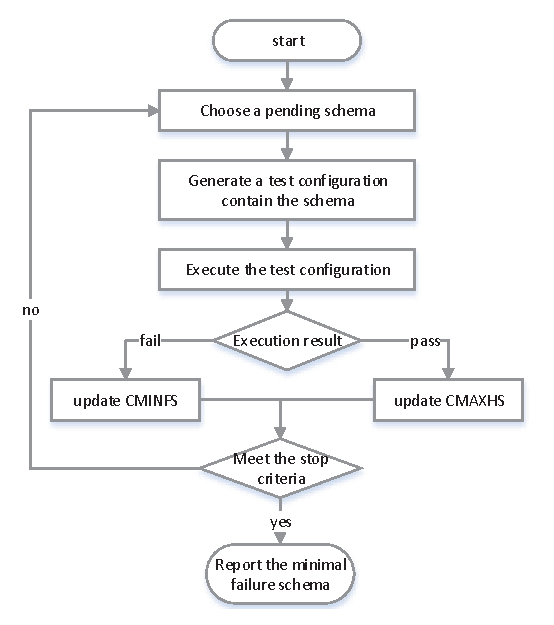
\includegraphics[width=2.7in]{gp.eps}
 \caption{overview of approach of identifying MFS}
 \label{fig_overview}
\end{figure}
\subsubsection{Choosing a pending schema}
Before we think getting a pending schema, we should assume an general scenario. That is, we have already make sure some schemas to be healthy schemas and some schemas to be faulty schemas, then assume that we still don't meet the stopping criteria, we will choose a pending to check next. But first, we should make sure what schema is pending schema?

In effect, the schemas we can't make sure whether are faulty schemas nor healthy schemas are our wanted. Step further, we sperate this condition into two parts: 1. can't make sure it is faulty schema. As we already know some faulty schemas, then we just make the schema that first not be any one of these faulty schemas and not be the parent-schema of any one of these faulty schemas(As if not, it must be a faulty schema according to the proposition 3). 2 can't make sure it is healthy schema. Similar to the first condition,we already know some healthy schemas, then we just make the schema that first not be any one of these healthy schemas and not be the subschema of any one of these healthy schemas. It is obvious a pending schema must meet both the two conditions.

However, this is not the end of story of checking a pending schema. With the process of identifying, more and more faulty schemas and healthy schemas will be identified. It is not a small number, as it can reach to O($2^n$). So both for space and time restriction, we should not record all the faulty schemas and heathy schemas. Then we should find another way to check the pending schema.

To eliminate this problem, we propose an method which can check a pending schema with a small cost. It need to record the CMINFS and CMAXHS all through the process. Instead record all the faulty schemas and healthy schemas, CMINFS and CMAXHS are rare in amount, which can help to largely reduce the space need to record. Then according to the followed two propositions, we can easily check a pending schema.

\begin{proposition}
If a schema is neither one of nor the parent-schema of any one of the CMINFS, then we can't make sure whether it is a faulty schema.
\end{proposition}
\begin{proof}
Take a schema $s_a$, a CMINFS set $S_{cminfs}$ and a faulty schema $S_{fs}$ set which determined now. It is note that any element $fs_i \in S_{fs}$ must meet that either $fs_i \in S_{cminfs}$ or $fs_i$ be the parent-schema of one of the $S_{cminfs}$. Assume that $s_a$ is neither the one of nor the parent-schema of any one of the $S_{cminfs}$. To proof the proposition, we just need to proof that $s_a$ is neither the one of nor the parent-schema of any one of the $S_{fs}$.

As $s_a$ is neither the one of nor the parent-schema of any one of the $S_{cminfs}$, so it is not one of $S_{fs}$. Then we assume $s_a$ is the parent-schema of one of $S_{fs}$, say, $fs_j$. As $fs_j$ must meet either $fs_j \in S_{cminfs}$ or $fs_j$ be the parent-schema of one of the $S_{cminfs}$. So $s_a$ is the parent-schema of one of $S_{cminfs}$ according to the proposition 2, which is contradict. So the proposition is correct.
\end{proof}

\begin{proposition}
If a schema is neither one nor the the subschema of any one of the CMAXHS, then we can't make sure whether it is a healthy schema.
\end{proposition}
We ignore this proof as it is very similar to the previous one.

Up to now, we can judge whether a schema is a pending schema, but in effect, there are many pending schemas in a test configurations, especially at the beginning of our process. To choose which one has an impact on our approach. To better illustrate this problem, we consider the followed example:

Assume the failing test configuration: (1 2 1 1 1 2 1 2), that the CMINFS set: (1 2 1 1 - 2 - -) (- 2 - - 1 2 - 2), the CMAXHS set:(- 2 - - - - - -) (- - - - 1 - - -). We list some pending schemas followed (not all, as the number of all the pending schemas is too much that is not suitable to list here):

(1 2 1 - - 2 1 2) (- 2 1 1 - 2 - 2) (1 2 1 1 - - - -) (- 2 1 1 - 2 - -) (1 2 1 - - - - -) (- 2 - 1 - - 2 -) (1 2 - - - - - -) (- - 1 1 - - - -) (1 - - - - - - -)  (- - 1 - - - - -).

Choose what is really different. If we choose (1 2 1 - - - - -), assume we check it as a healthy schema. Then all its subschemas, such as (1 2 - - - - - -) (1 - - - - - - -)  (- - 1 - - - - -), are healthy schemas. It means that we did not need generate newly test configurations for them. But if we check it as a faulty schema, we can make sure all its parent-schemas are faulty schemas, in this case, they are (1 2 1 1 - - - -) and (1 2 1 - - 2 1 2) need no newly test configurations to test.

Let's look at this problem from another angle. Take the schema as a integer number, these parent-schemas of a schema is like the integer numbers bigger then this number, and these subschemas of a schemas is like the numbers smaller than this number. Take a float number as the metric, then, we can describe the faulty schema as the number bigger than this metric, and healthy schema as number smaller than this metric. So the minimal faulty schema is just the number most approximate the metric and bigger than the metric.

It seems like a search problem scenario. Then can we directly apply the efficiently algorithm binary-search? the answer is no, because there are schemas that neither parent-schema or subschema relationship, such as(1 2 1 - - 2 1 2) (- 2 1 1 - 2 - 2). So to utilize the binary search technique, we should make some change. First, should give the followed definitions:

\begin{definition}[chain]
A chain is an ordered sequences of schemas in which every schemas is the direct parent-schema of the schema that follows. Moreover,if all the schemas in a chain are pending schemas, we call the chain a pending chain.
\end{definition}
This definition is similar to the path in []

As all the schemas in a chain are have relationships, then we can apply binary search technique. As we all know, the longer the pending chain, the better performance binary search technique will get. So we should choose a pending chain as longer as possible each iteration.

To get a longest chain, we need to ensure that the head schema of this chain do not have any parent-schema which is a pending schema(called up pending schema), and the tail schema do not't have any subschema which is a pending schema (called down pending schema). The algorithm that get the up pending schemas and down pending schemas are list in algorithm 1 and algorithm 2.

As showed in algorithm 1, we start from the failing test configuration $\mathcal{T}$, assign it to the \emph{rootSchema}(line 1)and then add it to a \emph{lists}(line 3). We then do some operation (line 4 -line 12)to this lists and at last get these pending schemas in lists as up pending schemas.(line 13)  This operation consists of two iteration:

1. successively get one \emph{CMINFS} in $\mathcal{S_{CMINFS}}$. (line 4). Define a temple value \emph{nextLists} which initialize an empty set(line 5).We then execute the second iteration. After that, we will eliminate these same schemas list in \emph{nextLists} (line 10)and then assign to \emph{lists} (line 11).

2. Successively get one schema in \emph{lists}(line 6). And then mutant it according to the \emph{CMINFS} to a set of schemas(line 7). Add them to the  \emph{nextLists} (line 8).

The mutant procedure for a schema is just remove one value in it which this value is also in \emph{CMINFS}. This procedure will result in \emph{k} mutant schemas if the \emph{CMINFS} is a \emph{k}-value schema. By doing this, any mutant schema will not be the parent-schema of the corresponding \emph{CMINFS}.

After this two iteration, the schemas in the \emph{lists} will not be the parent-schema of any \emph{CMINFS} in the $\mathcal{S_{CMINFS}}$.

\begin{algorithm}
  \caption{getting up pending schema}
  \begin{algorithmic}[1]
     \Require  $\mathcal{T}$ \Comment{failing test configuration}

     $\mathcal{S_{CMINFS}}$ \Comment{set of CMINFS}

     $\mathcal{S_{CMAXHS}}$ \Comment{set of CMAXHS}

     \Ensure  $\mathcal{S_{UPS}}$ \Comment{the set of up pending schemas}

    \Statex\Comment{\%comment: initialize\%}
    \State $rootSchema \leftarrow \mathcal{T}$
    \State $lists \leftarrow \emptyset$
    \State $lists \cup \{rootSchema\}$

    \ForAll{$CMINFS$ in $\mathcal{S_{CMINFS}}$}
     \State $nextLists \leftarrow \emptyset$
     \ForAll{$schema$ in $lists$}
        \State$S_{candidate} \leftarrow mutant_{r}(schema,CMINFS)$
        \State $nextLists \leftarrow nextLists \cup S_{candidate}$
     \EndFor
     \State $compress(nextLists)$
     \State $lists \leftarrow nextLists$
    \EndFor
     \State $\mathcal{S_{UPS}} \leftarrow   \{ s | s \in lists \wedge {s\ is\ pending}\}$
  \end{algorithmic}
\end{algorithm}

Fig.\ref{figch} gives an example to the algorithm 1.

\begin{figure}
 \centering
 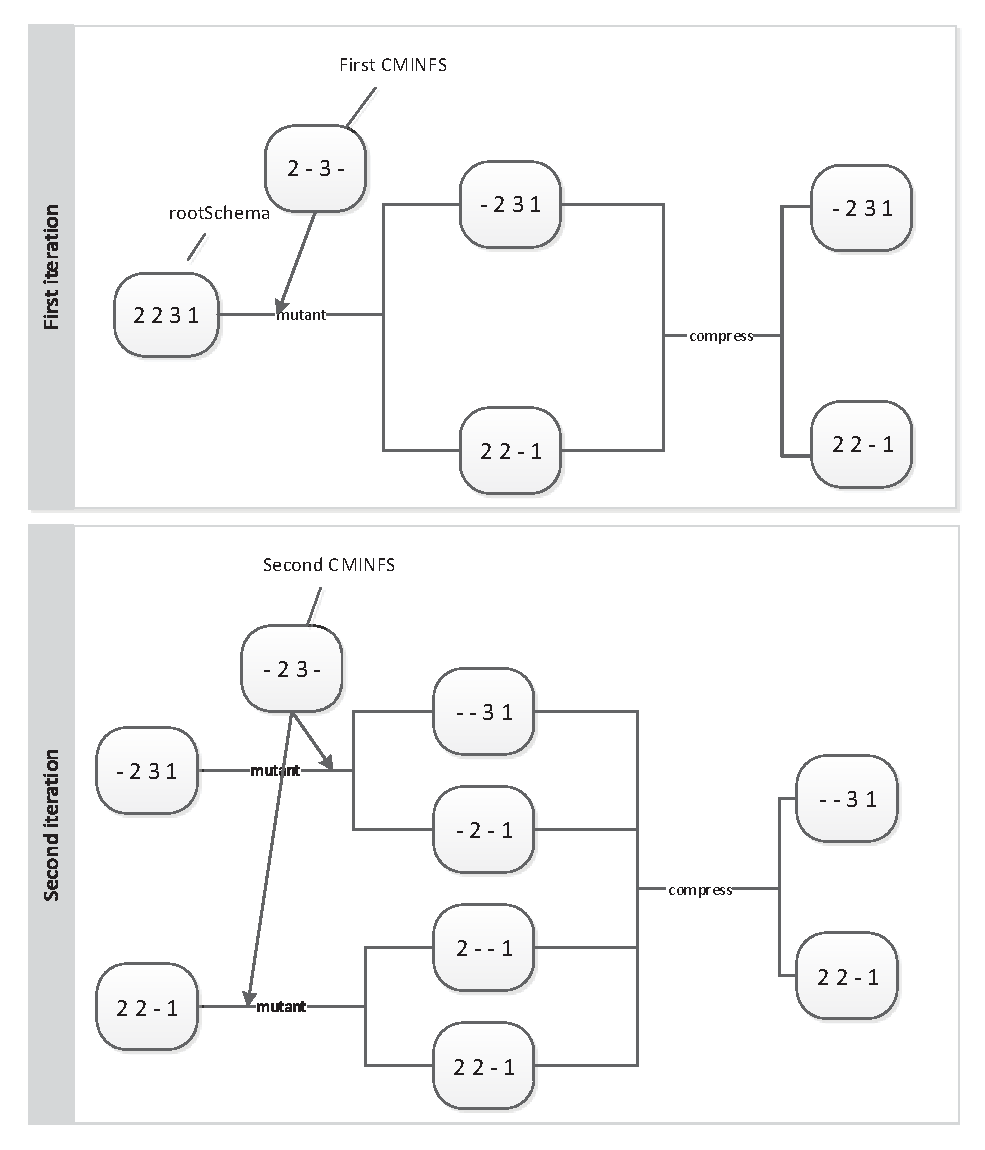
\includegraphics[width=2.8in]{ch.eps}
 \caption{example of getting up pending schemas}
 \label{figch}
\end{figure}


Algorithm 2 is a bit different from algorithm 1. As our target is to get the minimal value pending schema, we get started from a 0-value schema(line 1). Then to make schemas not to be the subschema of any \emph{CMAXHS} in $\mathcal{S_{CMAXHS}}$, we should let the schemas must contain at least one value that is not in the corresponding \emph{CMAXHS}. So the strategy is to get a reverse schema of the \emph{CMAXHS} which this schema consists of all these values in the failed configuration except these are in \emph{CMAXHS}(line 5). And mutant the schema by adding one value in the reversed schema to make the schma not to be the subschema of the correspinding \emph{CMAXHS}(line 8). After two iteration similar to Algorithm 1, we will get all the schemas that meet that not to be  subschema of any \emph{CMAXHS} in $\mathcal{S_{CMAXHS}}$ from which we choose these pending schemas as down pending schemas(line 14).


\begin{algorithm}
  \caption{getting down pending schema}
  \begin{algorithmic}[1]
     \Require  $\mathcal{T}$ \Comment{failing test configuration}

     $\mathcal{S_{CMINFS}}$ \Comment{set of CMINFS}

     $\mathcal{S_{CMAXHS}}$ \Comment{set of CMAXHS}

     \Ensure  $\mathcal{S_{DOWNS}}$ \Comment{the set of down pending schemas}

    \Statex\Comment{\%comment: initialize\%}
    \State $initschema \leftarrow \mathcal{()}$
    \State $lists \leftarrow \emptyset$
    \State $lists \cup \{initschema\}$

    \ForAll{$CMAXHS$ in $\mathcal{S_{CMAXHS}}$}
     \State $reverse \leftarrow \ reverse(CMAXHS)$
     \State $nextLists \leftarrow \emptyset$
     \ForAll{$schema$ in $lists$}
        \State$S_{candidate} \leftarrow mutant_{a}(schema,reverse)$
        \State $nextLists \leftarrow nextLists \cup S_{candidate}$
     \EndFor
     \State $compress(nextLists)$
      \State $lists \leftarrow nextLists$
    \EndFor
     \State $\mathcal{S_{DOWNS}} \leftarrow   \{ s | s \in lists \wedge {s\ is\ pending}\}$
  \end{algorithmic}
\end{algorithm}

Fig.\ref{figct} gives an example to the algorithm 2. we can see.
\begin{figure}
 \centering
 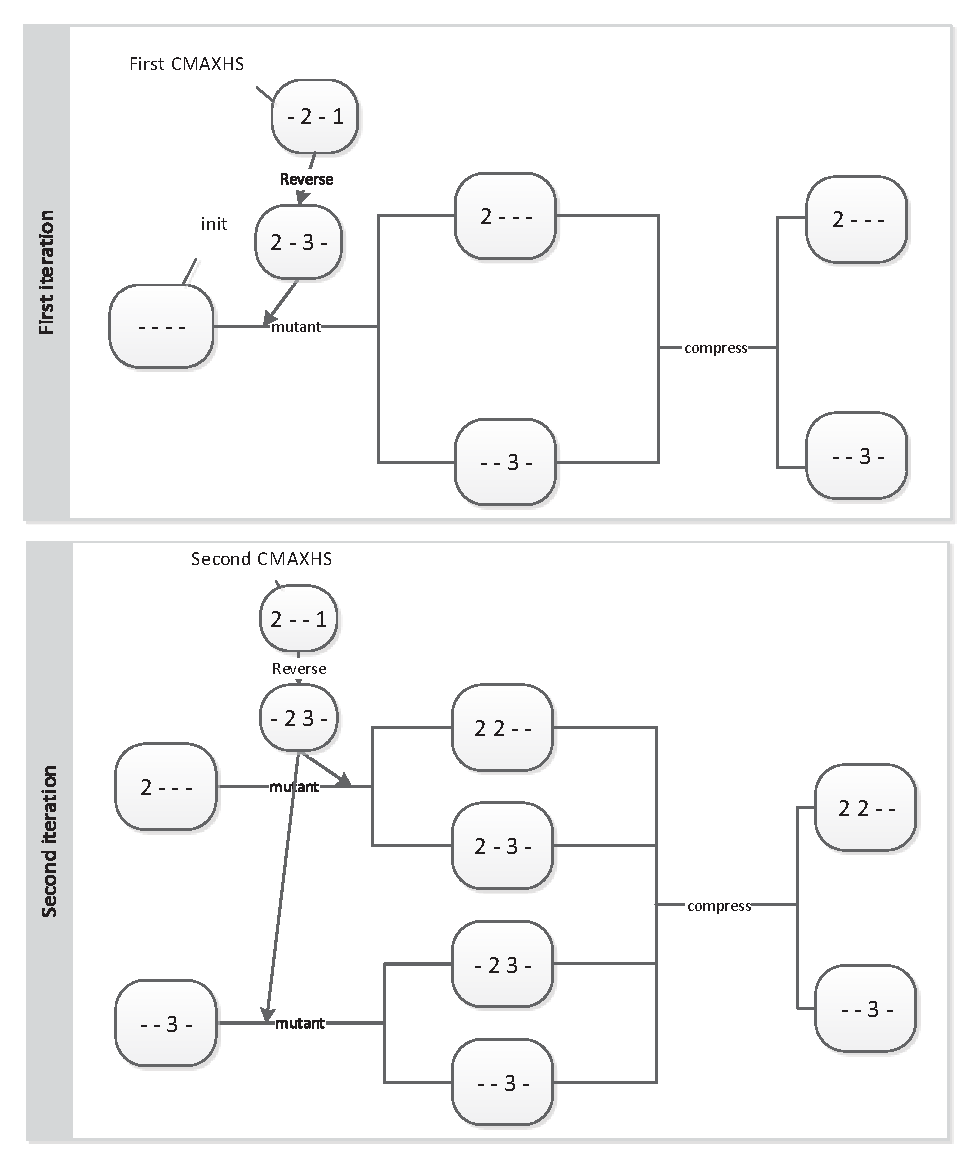
\includegraphics[width=2.8in]{ct.eps}
 \caption{example of getting down pending schemas}
 \label{figct}
\end{figure}

After we can get the up pending schemas and down pending schemas, then the algorithm of getting the longest chain can be very simple,which is list in Algorithm 3. In this algorithm we can see that we just search through the up pending schemas and down pending schemas(line 7 - 8) to find the two schemas which has the maximum distance(line 9 - 13). The distance of a k-value schema and a l-value schema (k>l) is defined as:

$$distance(S_k, S_l) =
\begin{cases}
-1, & S_k\ is\ not\ parent-schema\ of\ S_l\\
k-l,& otherwise
\end{cases}
$$

Then we just use \emph{makechain} procedure to generate the longest chain. The \emph{makechain} procedure is very simple, it just repeat adding one schema by keeping all the value in down pending schema and removing one factor of the previous schema.

\begin{algorithm}
  \caption{Finding the longest pending schema}
  \begin{algorithmic}[1]
     \Require  $\mathcal{T}$ \Comment{failing test configuration}

     $\mathcal{S_{CMINFS}}$ \Comment{set of CMINFS}

     $\mathcal{S_{CMAXHS}}$ \Comment{set of CMAXHS}

     \Ensure  $\mathcal{CHAIN}$ \Comment{the chain}
    \State $\mathcal{S_{UPS}} \leftarrow getUPS(\mathcal{T},\mathcal{S_{CMINFS}},\mathcal{S_{CMAXHS}}) $
    \State $\mathcal{S_{DOWNS}} \leftarrow getDOWNS(\mathcal{T},\mathcal{S_{CMINFS}},\mathcal{S_{CMAXHS}}) $
    \State $max \leftarrow 0$
    \State $head \leftarrow NULL $
    \State $tail \leftarrow NULL $
    \State $chain \leftarrow NULL $
     \ForAll{$up$ in $S_{UPS}$ }
        \ForAll{$down$ in $S_{DOWNS}$}
            \If {$distance(up, down) \geq max$}
              \State $max \leftarrow distance(up, down)$
              \State $head \leftarrow up$
              \State $tail \leftarrow down$
             \EndIf
        \EndFor
     \EndFor
     \State $\mathcal{CHAIN} \leftarrow  makechain(head, tail)$
  \end{algorithmic}
\end{algorithm}

The last step of getting the schema is just choose the schema from the longest chain. To clearly describe the approach, we discuss it in the overall identifying algorithm which is list in the Algorithm 4. As we have talked previously, we first judge the end criteria, if meet we will report the minimal faulty result. Otherwise we will do the loops. In the loop, we first judge if it is the beginning or headIndex greater than tailIndx, then we will update the CMINFS and CMAXHS, followed generated the longest chain and initial the headIndex, tailIndex and middleIndx. If not we will get the middleIndex indicate the half. Then will select the schema with index of middleindex in the longest chain. And then generate a test configration and exectute the SUT under it. If the result passed, we let tail = middle - 1 else head = middle + 1. By doing this and the previous set the middleIndex we can apply the binary searh to the indentying. It is noted that we intitally let middle = 0. which we want know if this chain has faulty schema as soon as possible.
\begin{algorithm}
  \caption{identify process}
  \begin{algorithmic}[1]
    \Require  $\mathcal{T}$ \Comment{failing test configuration}

     $\mathcal{S_{CMINFS}}$ \Comment{set of CMINFS}

     $\mathcal{S_{CMAXHS}}$ \Comment{set of CMAXHS}

     \While{$hasn't\ meet\ the\ end\ criteria$}
       \If{$the\ beginning$ or $headIndex > tailIndex$}
       \State $update(\mathcal{S_{CMINFS}},\mathcal{S_{CMAXHS}})$
       \State $longeset \leftarrow getLongest( \mathcal{T},\mathcal{S_{CMINFS}},\mathcal{S_{CMAXHS}})$
       \State $headIndex \leftarrow 0$
       \State $tailIndex \leftarrow length(longest) - 1$
       \State $middleIndex \leftarrow 0$
     \Else
       \State $middleIndex \leftarrow \frac{1}{2} \times (tailIndex + headIndex)$
     \EndIf
       \State $\mathcal{SCHEMA} \leftarrow longest[middleIndex]$
       \State $generate\ a\ extra\ test\ configration\ \mathcal{T'}\ contain\ \mathcal{SCHEMA}$
       \State $execute\ SUT\ under\ \mathcal{T'}$
     \If{$the\ test\ configration\ passed$}
       \State $tailIndex \leftarrow middleIndex - 1$
     \Else
       \State $headIndex \leftarrow middleIndex + 1$
     \EndIf
   \EndWhile
   \State $report\ the\ minimal\ faulty\ schemas$
  \end{algorithmic}
\end{algorithm}

\subsubsection{generate a new test configuration}
To generate a new test configuration to test the schema. The generated test configuration must meet the followed rules:

1. must contain the selected schema.

2. must not

3. constraint(system-wide constraint and test case specific constraint, i.e., masking effect)

The first one is easy to meet. We just keep the same value which are in the schema are also in the test configuration.
We must meet the second condition for that if we contain another one, combine this then this test configuration will contain an parent-schema of this selected schema in the original test configuration, and it will confuse us whether it is indicate this schema or its parent-schemas dedicate this result. To fulfil this condition, we need to choose other available values in the SUT which are different from the original test configuration.
the third one is that we should consider the constraints

\subsubsection{execute SUT under the test configuration}
In real software testing scenario, when we test a SUT under a test configuration, there may be many possible testing state: such as pass the testing assertion, don't pass the testing the assertion but with different failure type, can't complete the testing. To get a clear discussion, in this paper we just use \emph{pass} represent the state that pass the testing assertion and \emph{fail} represent all the remained state.

\subsubsection{update information}
The update information is followed when the current chain is checked over. Then before we generate another longest chain, we should update the CMINFS and CMAXHS set. In fact, we just need the CMINFS and CMAXHS in the longest chain.

\subsubsection{stop criteria}
The stop criteria is clear, our algorithm stops when there are no pending schemas left, for that when we once can checked all the schemas of a test configuration, we can get the minimal faulty schemas, which is the target of our algorithm. And whether there are pending schemas can be easily checked by that if we can't generate a longest chain (the length must greater than 1), there must be no pending schemas.
\subsubsection{report the reuslt}
In fact, the last in the CMINFS lists is must be the minimal faulty schemas. For that if these schema in the CMINFS is not minimal faulty schema, then there must be some pending schemas. However, the algorithm stop when there are no pending schemas remained. So at last these in the CMINFS must be the minimal faulty schemas.

\subsubsection{new ideas}
you should first identify a failure-inducing schema, and then find others. initial the find tuples, and then using the same algorithms as others. when identify is confirm ,  then choosing new longest path.

\subsection{example}
We will give an complete example listed in Table \ref{identifying_example}. Assume that a SUT is . constaints.
\begin{table*}\renewcommand{\arraystretch}{1.3}
  \caption{An example of identifying} \centering
  \label{identifying_example}
  \begin{tabular}{c|c|c|c|c|c}\hline
  \hline
  \bfseries $\mathcal{S_{CMINFS}}$ &   \bfseries $\mathcal{S_{CMAXHS}}$ & \bfseries Longest Chain & \bfseries Choosing Schema & \bfseries Generating Test Configuration & \bfseries Execution result\\
  \hline
  1 & 1 & 1 & 1 & 1 & false \\
   1 & 1 & 1 & 1 & 1 & pass\\
  1 & 1 & 1 & 1 & 1 & false\\
  \hline
  \end{tabular}

\end{table*}

\subsection{Without Safe Values Assumption}
Up to now our algorithm is based on the assumption that additional generated test configuration does not introduce newly faulty schema. We will give an augment algorithm this section to eliminate this assumption.
Our augment algorithm is inspired by the feedback machinery in the controlling system, which in high level we will validate the identify result at the end of the aforementioned algorithm, and if the schema is validated as a minimal faulty schema, we will end the algorithm, otherwise we will repeat the algorithm again to adjust the result. The detail of our augment algorithm is list in Algorithm 5. We can find the first part of augment algorithm is an unlimited loop, in the loop we first use previous identify algorithm to identify the MFS, and then we will check the result, the check process is just to addtional generate another test configurations and execute. When we find the MFS is not right, which means our process introduce newly MFS, then we first label this MFS as an healthy schema, and then update the CMAXHS. After check, if we find at least one MFS is not right, we then empty the CMINFS, and then readd these right identified MFS to this set, and then reprocess this process untill all the MFS is validated as right. The second part of our algorithm is just we look through the generated test cases one by one, if it failed, and did not contain the MFS we identified in the first part, which means it introduce newly faulty schema, and we will rerun this process to find these introduced MFS.
\begin{algorithm}
  \caption{augment identify process}
  \begin{algorithmic}[1]
    \Require  $\mathcal{T}$ \Comment{failing test configuration}

     $\mathcal{S_{CMINFS}}$ \Comment{set of CMINFS}

     $\mathcal{S_{CMAXHS}}$ \Comment{set of CMAXHS}

     \While{$true$}
       \State $\mathcal{S_{MFS}} = Identify\_process(\mathcal{T})$
       \ForAll{$MFS$ in $\mathcal{S_{MFS}}$}
       \If{$validate(MFS) = fail$}
         \State $updateHealthySchemas(S_{CMAXHS},MFS)$
       \EndIf
       \EndFor
       \If{$at\ least\ one\ MFS\ is\ not\ correct$}
          \State $empty(S_{CMINFS})$
          \State $add\ all\ the\ vaildated\ MFS\ in\ the \mathcal{S_{CMINFS}}$
       \Else
           \State $break$
       \EndIf
      \EndWhile
      \ForAll{$testCase$ in $\mathcal{EXTRATESTCASES}$}
         \If{$testCase\ introduce\ newly\ MFS$}
           \State $augment\_identify\_process(testCase)$
         \EndIf
      \EndFor
      \State $report\ the\ minimal\ faulty\ schemas$
  \end{algorithmic}
\end{algorithm}

Table \ref{augment_example} illustrate this augment algorithm with an example.
\begin{table*}\renewcommand{\arraystretch}{1.3}
  \caption{An example of augment identifying} \centering
  \label{augment_example}
  \begin{tabular}{c|c|c|c|c|c}\hline
  \hline
  \bfseries $\mathcal{S_{CMINFS}}$ &   \bfseries $\mathcal{S_{CMAXHS}}$ & \bfseries Longest Chain & \bfseries Choosing Schema & \bfseries Generating Test Configuration & \bfseries Execution result\\
  \hline
  1 & 1 & 1 & 1 & 1 & false \\
   1 & 1 & 1 & 1 & 1 & pass\\
  1 & 1 & 1 & 1 & 1 & false\\
  \hline
  \end{tabular}

\end{table*}

\section{Evaluation using simulated model}
In this section, we give an a series of  studies of our two identify algorithms on simulated model. The goal of our experiments is to evaluate the efficiency and effectiveness of our two identify algorithms compared with other existed algorithms. The reason why we use simulated model is that we can control. We will validate in real softwares in the next section.
\subsection{comparison algorithms}
There are some algorithms aim to identify the MFS, they can be classified as non-adaptive methods and adaptive methods. The first set of methods do not need additional test configurations and can identify the when given an executed test configurations while the second one do need. Our algorithm is belong to the second part. To make a clear comparison, we just compare the algorithms which all belong to this part.vThe more detail and discuss of all the algorithms is listed in the section 6. The compared algorithms is as follows:
\subsubsection{OFOT}
This method is proposed by Nie[]. It first separates the faulty-possible tuples and healthy-possible tuples into two sets. Subsequently, by changing a parameter value at a time of the original test configuration, this approach generates extra test configurations. After executing the configurations, the approach converges by reducing the number of tuples in the faulty-possible sets.
\subsubsection{IterAIFL}
This method proposed by Wang[] is a mutant based ont the Nie's[]. It define the "change strength" that not like the previous one just change one factor one time, it may change many factors one time.

\subsubsection{FIC}
Zhang [] propose this method which is combined the OFOT method and binary search. Different from the OFOT, it change half factor one time to quickly located in one factor firstly and then keep the factor and loop the process.

\subsubsection{RI}
Lee propose this algorithm[]. Similar to the FIC, it is also inspired by the delta debugging. The difference is the order that it change factors.

\subsubsection{Spetrum based method}
Different from the aforementioned methods, Ghandehari.etc [10] defines the suspiciousness of tuple and suspiciousness of the environment of a tuple. Based on this, they rank the possible tuples and generate the test cases. Although their approach imposes minimal assumption, it does not ensure that the tuples ranked in the top are the faulty tuples.

the parameter setting is as follows: the predefined number is 5, and the number of turns of finding the minimum pe is the parameter mutipled.
\subsubsection{Martin safe value}


\subsubsection{classified tree}
must add "-M 1" "-U" confidence factor 0.25

\subsubsection{TRT}
This algorithm is proposed in[].Different from this work. It should record all the schemas of a failed test configuration. It is very resource assume and this is reason we propose this work. A second difference is that the TRT algorithm when meet the situation the extra test configuration may introduce newly faulty schemas is using more test configuration to confirm a schema each time when find a schema is labeled as a faulty schema while this work just validate one time at the end of algorithm.

\subsection{subject programs}
This section will give an general illusion of the algorithms. We will give an test bench to measure the properties of all the algorithms. All the programs are toys and have the property that we can easily control its input parameters and faulty schemas, which makes clearly get the view of what we want to know from the algorithms. In addition, we will corroborate the results by observing each algorithm of identifying failure-inducing schemas in real software in section 6.

\subsection{evaluation metrics}
The metrics are additional generated test configurations, the recall and precise.The recall and precise  is defined as:

$$recall =
 \frac{Identiied\ MFS}{all\ the\ MFS\ in\ SUT}
$$

$$precise =
 \frac{correctly\ Identified\ MFS}{all\ the\ identified\ MFS}
$$
\subsection{experiment setups}
We will do the three experiment: (1)single faulty schema.  (2)multiple faulty schema in a failed test configuration. (3)multiple faulty schema, which give a fail test configuration contain one faulty schema , we do so that give an chance that the extra test configuration can introduce another faulty schema.

In detail, for every experiment in the toy experiment section, we first vary the number of input parameters of SUT, i.e., \emph{n}= 10, 40, 80, 120, 160, 200, 240, 280, 320, 360 to observe the behaviour of the algorithms executed among different size of SUT. Then to get an relative generally evaluation, we inject each possible \emph{t}-value schema (reach to $\binom{n}{t}$,) one time for the single faulty schema experiment and each possible combination of two \emph{t}-value schema one time for the multiple faulty schema experiment.(t = 2,3,4,5,6). For the third, we first fix one \emph{t}-value faulty schema, and give an failed test configuration contain this schema, then for each algorithm aims to identify this faulty schema, the first extra test configuration each algorithm generate, we random select an \emph{t}-value schema (do not contained in the original failing test configuration) as the introduced faulty schema.

For all the three experiment, we record the number of extra test configurations, correctly identified schemas and incorrectly identified schemas. At last we compute the recall and presise along with the number of extra test configurations.

%\begin{table}\renewcommand{\arraystretch}{1.3}
%  \caption{The set up of toy  experiment} \centering
%  \label{toy-experiment}
%  \begin{tabular}{c|c|c|c}\hline
%  \hline
%  \bfseries categories & \bfseries version No  & \bfseries LOC  & \bfseries input model\\
%  \hline
%   MySQL & 2013121 & 1 & $2^{2}\times3^{2}$\\
%     \ & 2013121 & 1 & $2^{2}\times3^{2}$\\
%     \ & 2013121 & 1 & $2^{2}\times3^{2}$\\
%     \ & 2013121 & 1 & $2^{2}\times3^{2}$\\
%   FireFox & 2013121 & 1 &  $2^{2}\times3^{2}$\\
%     \ & 2013121 & 1 & $2^{2}\times3^{2}$\\
%     \ & 2013121 & 1 & $2^{2}\times3^{2}$\\
%  \hline
%  \end{tabular}
%\end{table}
\begin{figure}
 \centering
 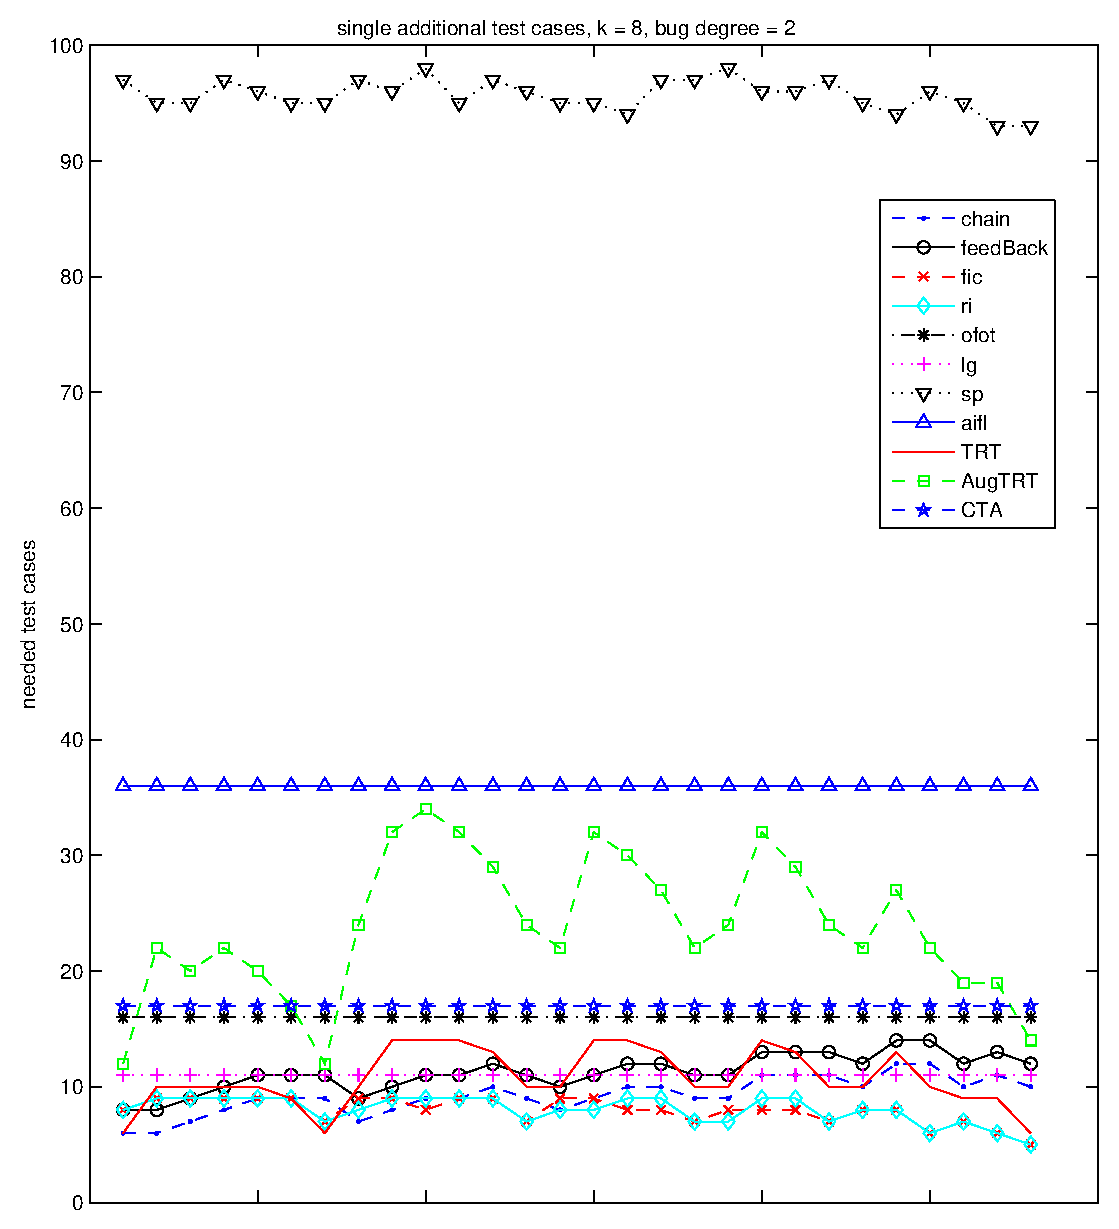
\includegraphics[width=2.8in]{single.eps}
 \caption{k = 8, t = 2, additional test suites}
 \label{fig_single}
\end{figure}

\subsection{results and discuss}

\subsection{threats to validate}
how seeded bugs are representative
auto oracle, if we don't have a correct version, or we can't determine a test case is faulty and wrong, then what can i do?
timing result
One worrying aspect of this research is that it seems to consider only the number of tests and number of faults uncovered. In the practice of testing, it is as important or more important to know testing times.

\section{Empirical Case study}
 While we got know that our approach have a better performance than others in several scenarios such as a failing test case contains multiple MFSs, the generated extra test case introduces newly MFS and so on from previous simulated experiments, it did not give us strong confidence in that our approach will also perform well in real software systems. One important reason of this is that we don't know whether these competitive scenarios for our approach existed in real software systems. So to eliminate the doubt we conduct a series empirical studies in this section. These empirical studies aimed to answer the following questions:

 Q1:Is there any test case that contain multiple MFSs, and if so, do they overlapped each other? Do any of these MFSs have high degree and how likely does it introduce newly MFS when generate extra test cases.

 Q2:How well of these approaches mentioned in previous sections performed when identifying the MFS in the real softwares?

 Q3:If we combine the result of one approach with another one, does it give us a better result than both of them?

The subject systems for these studies are HSQLDB(2.0rc8). HSQLDB is a database management system written in pure java. All of them have millions of uncommented lines of code. And they all share the same proceedings depicted in Fig.\ref{proceeding} when tested in the following studies.
\begin{figure}
 \centering
 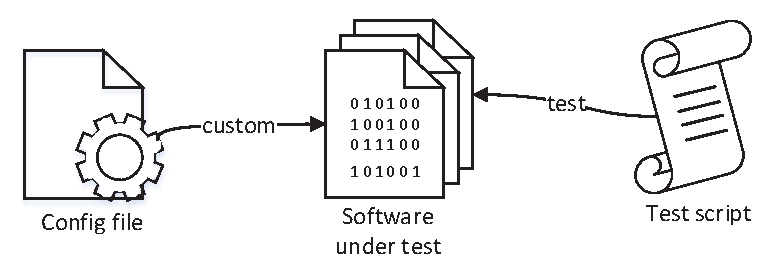
\includegraphics[width=2.7in]{proceed.eps}
 \caption{proceeding}
 \label{proceeding}
\end{figure}

As see from the figure, there are three modules in this proceeding: configuration file, software under test and the test script. The software under test is a set of software components which supply some interfaces, with which one can invoke the serving functions of the software. The configuration file is the file that can custom the properties of the software, and the test script is a executable file which test some functions of the software. In specific, the proceeding is trying different configuration of the software by changing the content of the configuration file, and then executing the same test script to observe the result.

\subsection{experimental setup}
Before we use these programs for study, we will take the following steps for each program to obtain the basic information of them, 1)Build the input configuration model of the subject program 2)execute the test case under each possible configuration and record their executed result. 3)list all the types of fault during testing and judge their priority.

We will depict these processes and results for each subject program in detail.
\subsubsection{HSQLDB}
Through searching the developers' community of HSQLDB in sourceforge, we found a buggy version with its faulty description in [], and a test script is attached which can reproduce the bug. The original test script only considered one option which have two values, remaining the other options set default values. To see what will happen when executing the test script under more different configurations, we need add some other options which may influence the behaviour of the database management software. From numerous optioins of HSQLDB, We chose some of the options that control the properties of table, some control the sql, some control the server and some control the result set. Along with the one in the original test script, we derive a input configuration model of HSQLDBlisted in table \ref{modelHSQLDB}.

\begin{table}\renewcommand{\arraystretch}{1.3}
  \caption{input model of HSQLDB} \centering
  \label{modelHSQLDB}
  \begin{tabular}{p{0.9\columnwidth}}\hline
  \hline
   \bfseries  SQL  properties(TRUE/FALSE)\\
    \hline
    sql.enforce\_strict\_size, sql.enforce\_names,sql.enforce\_refs, sql.enforce\_size, sql.enforce\_types, sql.enforce\_tdc\_delete, sql.enforce\_tdc\_update
  \end{tabular}

  \begin{tabular}{c*{2}{p{0.53\columnwidth}}}
  \hline
  \bfseries table properties &   \bfseries values \\
   \hline
   hsqldb.default\_table\_type & CACHED, MEMORY\\
   hsqldb.tx & LOCKS, MVLOCKS, MVCC\\
   hsqldb.tx\_level & read\_commited, SERIALIZABLE\\
   hsqldb.tx\_level & read\_commited, SERIALIZABLE
  \end{tabular}

  \begin{tabular}{c*{2}{p{0.53\columnwidth}}}
  \hline
  \bfseries Server properties &   \bfseries values \\
   \hline
   Server Type & SERVER, WEBSERVER, INPROCESS \\
    existed form & MEM, FILE
  \end{tabular}

  \begin{tabular}{c*{2}{p{0.53\columnwidth}}}
  \hline
  \bfseries Result Set properties &   \bfseries values \\
   \hline
    resultSetTypes & TYPE\_FORWARD\_ONLY,TYPE\_SCROLL\_INSENSITIVE, TYPE\_SCROLL\_SENSITIVE\\\
    resultSetConcurrencys & CONCUR\_READ\_ONLY,CONCUR\_UPDATABLE \\
    resultSetHoldabilitys & HOLD\_CURSORS\_OVER\_COMMIT, CLOSE\_CURSORS\_AT\_COMMIT
  \end{tabular}

  \begin{tabular}{c*{2}{p{0.53\columnwidth}}}
  \hline
  \bfseries option in test script &   \bfseries values\\
   \hline
   StatementType & STATEMENT, PREPAREDSTATEMENT
  \end{tabular}

\end{table}

%execute
We denoted this input model as ($2^{13}, 3^3$). There are $ 2^{13} * 3 ^ 3 = 221184 $ possible configurations in total. We executed the test script under each of the 221184 configurations and recorded their result. In specific, there are 147472 configurations triggered exceptions, while others passed this test. These exceptions can be classified to 4 types according to the exception traces. Through viewing the exception trace info and the source code of test script, we sorted out the priorities of these exceptions. Table \ref{faultyPriority} shows the detail of the 4 types of exceptions. The "exception ID" column shows the id of the exception. The "lower priority "column gives the IDs of exception which have lower priority than this exception. The "num of configs" means the number of test configurations under which the test script triggered this type of exception when executing.

%faulty type and their priority
\begin{table}\renewcommand{\arraystretch}{1.3}
  \caption{faulty and Priority} \centering
  \label{faultyPriority}

  \begin{tabular}{c*{3}{p{0.33\columnwidth}}}
  \hline
  \bfseries exception\ ID  &   \bfseries lower\ priority & \bfseries num\ of\ configs\\
   \hline
   1 & 2 & 36855\\
   2 & 1 & 110558\\
   3 & 1 2 & 58\\
   4 & 1 2 & 1
  \end{tabular}

\end{table}


\subsection{Study 1: what the schemas like in practice}
In the first study, we aimed to answer the Q1. We need to investigate the MFSs of the real softwares to see 1) Do there existed multiple MFSs in the same configuration? 2) if so, how many of them overlapped each other? 3) Do any of the MFSs have the degree larger than 2. 4) What the possibility of introducing newly MFSs when generating extra configurations. In particular we will inspect the MFSs in HSQLDB.

The first obstacle of case study 1 is that we don't know the MFSs in the real softwares. The original bug report page of these softwares[][] can give us hints of the MFSs of the software, but it is not enough for us to get accurate MFSs of the software. The reason is that we had added more options to test the script which resulted in more exceptions than reported and the original reported exception can also be related to more options that didn't be mentioned in the bug report.

So the only way to recognize the MFSs in the software is searching all the schemas in a configuration one by one, and then judging the state of the schema according to the definition and propositions. We will repeat the process in all the possible configurations of the software, this process is time-assuming which can be optimized by introducing hash table and adjusting the order when searching the schema of a configuration. We will omit these details as it is not point of this paper. Lastly after this time-assuming process we got the accurate MFSs for each software, we recorded them for later use.

\subsubsection{Measure the MFSs in the softwares}
As MFSs in the softwares are figured out, we can easily count the number of configurations contain multiples MFSs and MFSs that overlapped each other, as well as count the number of  MFSs that have a degree larger than 2.  But for the possibility of introducing newly MFSs when generating extra configuration (brief as possibility of introducing), we yet can't measure it for we didn't define how to compute the "possibility". We will give a formula to compute the possibility of introducing next, before then we will explain how is this formula derived.

First we should understand under which condition will the event of introducing newly MFSs harms our identifying algorithm.  Consider the following scenario.

For a test case of which we want to identify the MFS, say test case A,  if we change one factor of it to generate a new test case, say test Case B.  Then assume in this step we introduced a new failure-inducing schema, but meanwhile we didn't break the original failure-inducing schema in the test case A when we generate B, in other words, the MFS in A is still in B.

At this situation it will not influence our identifying result for that if we did not introduce the schema, our result is the same---trigger the same failure.

Consider another scenario, still for test case A, and we also change one factor of it to generate a new test case, say test Case C. Similarly, we introduced a new MFS, but different from the first scenario, this time we break the original MFS in the test case A when we generate C, which means the MFS in A is not in C.

At this situation it will influence our identifying result for that our expected result is that C should passed the test as we have broken the MFS in A. But the result failed at last. And we could owe this failure to some schema in A that is not the real MFS if we did nothing to deal with the introducing problem.

So we just need consider the possibility of the situation of simultaneously broking one MFS and introducing another MFS. This metric is related to the cost of changing one schema to another schema. The followed formula define the changing cost of two schemas:

ChangeCost(A, B) = $|T(A,B)| +\sum_{i \in T(B,A)}\left(P_{i} / 2\right) + \sum_{i \in S(A,B)}\left( |A_{i} - B_{i}| / 2\right)$

In this formula, A and B represent two different schemas. the denotation of T(A,B) gives the parameters in A but not in B. And S(A,B) means the parameters in both A and B, but their value is different.
$P_{i}$ refers to the number of values in the $i$th parameter of SUT, and $A_{i}$ is the value of one factor in Schema A , the factor is the $i$th parameter of SUT.

Then the introduce rate of a SUT is defined as:

$\dfrac {\sum_{a , b \in MFSs, a \neq b }\left(ChangeCost(a,b)\right)} {|MFSs|\times |MFSs - 1|}$

\subsubsection{result and analysis}
The statistic info of MFSs of the real software is listed in Table \ref{mfs-exp}.

\begin{table*}\renewcommand{\arraystretch}{1.3}
  \caption{MFSs information of each exception} \centering
  \label{mfs-exp}

  \begin{tabular}{c|c|c|c|c|c}
  \hline
  \bfseries exp\ ID  &  \bfseries MFSs & \bfseries degree\ than\ 2 & \bfseries mutliple\ MFSs& \bfseries overlapped\ MFSs &\bfseries intro rate\\
   \hline
   1 & 9 & 8 & 8 & 8 &0.1028\\
   2 & 24 & 23 & 25 & 1 &0.0145\\
   3 & 56 & 56 & 1 & 1 &0.0026\\
   4 & 1 & 1 & 0 & 0 & -
  \end{tabular}

\end{table*}

In this table,  "exp ID" is the id of exception which the MFSs will trigger, "MFSs" gives the number of MFSs that can trigger this type of Exception show in "exp ID" column. Column "degree than 2" list the number of MFSs that have a degree larger than 2.  "multiple MFSs" means the number of configurations that contain multiple MFSs. The column "overlapped MFSs" gives the number of configurations that contain MFSs that overlapped each other. And the last column "intro rate" shows the introduce possibility of newly MFSs when generating extra test configuration.

From this result, we will answer the sub-question of Case study 1 one by one.

1)Do there existed multiple MFSs in the same configuration?

Answer: yes. Although it is rare among the failing configurations(for exception 1, there are 36855 configurations trigger the same exception, and only 8 configurations contain multiple MFSs), but it do exist in the configurations of real software, we can see except the $4$th exception which just has one MFS, all the other exception have configurations have multiple MFSs, which are 8,25,1 respectively.

2)if so, how many of them overlapped each other?

Answer: most of them are overlapped each other. We learned configurations which have overlapped MFSs is 8, 1, 1 respectively. As we all know, the configurations have overlapped MFSs is just one part of the configurations have multiple configurations. Considering the configurations contain multiple MFSs is rare, which are 8 , 25, 1 respectively, then the  We think it is a high possibility when we encounter the situation that configurations contain multiple MFSs and these MFSs overlapped with each other.

One possible explanation for this phenomenon may be real softwares may have many branches, and these branches may have iteration, so for some MFSs , they may share the same entrance of the branch.

3)Do any of the MFSs have the degree larger than 2.

Answer: yes.  It is clearly that almost all the MFSs in the software have a degree than 2, except one MFS for exception 1 ( 8 among 9 MFSs have degrees larger than 2) and one MFS for exception 2( 23 among 24 MFSs have degrees larger than 2).

4)What the possibility of introducing newly MFSs when generating extra configurations?

Answer: the possibility varies from one to another.

We can learn from the table that the intro rate of exception 1 is 0.1028, which are the biggest than others, and the smallest is the exception 3, which is 0.0026. They differ markedly, so the possibility of introducing newly MFSs depends on the specific exception and may have big difference among each other.

\subsection{Study 2: how these algorithms behave when applied in real softwares}
The second study aims to answer the Q2. We will evaluate the performance of each algorithm in identifying the MFSs of the real softwares.
\subsubsection{Study setup}
To conduct this case study, for each algorithm. We will feed it with one failing configuration, for which we will use the algorithm to identify the MFSs. Then we will compare the result of this algorithm to the real MFSs in that configuration given in the study 1. The comparison metrics is similar to the simulated experiment, which consists of  the number of extra test configurations needed, the precise and the recall. To be fair, no other information is given to each algorithm except the feeded failing configuration. We will repeat this comparison for each failing configuration of a exception. At last we will report the average number of test configurations , precise and recall for each algorithm.

We will omit some algorithms which are time-consuming for identify these MFSs, it may need days even months, which is not available in practice. As the computing is very time-consuming, we just chose some algorithms mentioned in simulated experiment, they are ChainFeedBack , FIC, RI, OFOT, LG, CTA.

 \subsubsection{result and analysis}
 The result is show in table \ref{compare-casestudy}. In this table, Column "exp\ ID" still means for the specific exception of the ID. Column "algorithm" gives the specific algorithm measured in this row. Column "num of extra configs" shows the average number of extra configurations needed to generate to identify the MFSs. Column "recall" shows the recall and column "precise" shows the precise.

From the data listed in the table shows that our algorithm still perform better than others.
So the answer to Q2 is: the result in real softwares coincided with the result in simulated experiment.

 \begin{table*}\renewcommand{\arraystretch}{1.3}
  \caption{comparison in real softwares} \centering
  \label{compare-casestudy}

  \begin{tabular}{c|c|c|c|c}
  \hline
  \bfseries exp\ ID& \bfseries  algorithm   & \bfseries num\ of\ extra\ configs & \bfseries recall & \bfseries precise\\
   \hline
  1 & ChainFeedBack & 15.061 & 1.0 & 0.9995\\
  \  & FIC  &9.023& 0.9991 & 0.9988 \\
  \ & RI & 9.024 & 0.9991 & 0.9988 \\
  \  & OFOT &19.007 & 0.9997 & 0.9995 \\
  \  & LG &11.000 & 0.0 & 0.0\\
  \  & CTA &19.0 & 0.9997 & 0.9995\\
  \hline
  2 & ChainFeedBack & 13.058 & 0.9999 & 0.9996\\
  \  & FIC  &6.0160& 0.9999 & 0.9997 \\
  \ & RI & 6.0161 & 0.9999 & 0.9997 \\
  \ & OFOT &19.0 & 0.9997 & 0.9997 \\
  \  & LG &11.0005 & 0.9998 & 1.0\\
  \  & CTA &19.0 & 0.9997 & -\\
  \hline
  3 & ChainFeedBack & 19.793 & 0.9827 & 0.9827\\
  \  & FIC  &61.6551& 0.8879 & 0.89655 \\
  \ & RI & 62.6206 & 0.9396 & 0.9482 \\
  \ & OFOT &19.0 & 0.9827 & 0.9827 \\
  \  & LG &5.3448& 0 & -\\
  \  & CTA &19.0 & 0.9137 & 0.9137\\
  \hline
  4 & ChainFeedBack & 19.0 & 1.0 & 1.0\\
  \  & FIC  &65.0& 1.0 & 1.0 \\
  \ & RI & 65.0 & 1.0 & 1.0 \\
  \ & OFOT &19.0 & 1.0 & 1.0 \\
  \  & LG &5.0 & 0.0 & -\\
  \  & CTA &19.0 &1.0 & 1.0
  \end{tabular}
\end{table*}

 \subsection{Study 3: Is combination useful?}
 We can find from the last result, all of these algorithms can't all the time get good result. So a nature question is that can we combine the result of multiple algorithms and find a good result. In this study we will carry out some experiments to answer the question, i.e., the Q3.
 \subsubsection{Study setup}
 
 \subsubsection{result and analysis}

\section{Related works and Discuss}
Nie's approach in [3] and [6] first separates the faulty-possible tuples and healthy-possible tuples into two sets. Subsequently, by changing a parameter value at a time of the original test configuration, this approach generates extra test configurations. After executing the configurations, the approach converges by reducing the number of tuples in the faulty-possible sets.
Delta debugging [5] proposed by Zeller is an adaptive divide朼nd-conquer approach to locating interaction fault. It is very efficient and has been applied to real software environment. Zhang et al. [4] also proposed a similar approach that can identify the failure-inducing combinations that has no overlapped part efficiently,
Colbourn and McClary [7] proposed a non-adaptive method. Their approach extends the covering array to the locating array to detect and locate interaction faults.
C. Martiez [8-9] proposed two adaptive algorithms. The first one needs safe value as their assumption and the second one remove the assumption when the number of values of each parameter is equal to 2. Their algorithms focus on identifying the faulty tuples that have no more than 2 parameters.
Ghandehari.etc [10] defines the suspiciousness of tuple and suspiciousness of the environment of a tuple. Based on this, they rank the possible tuples and generate the test cases. Although their approach imposes minimal assumption, it does not ensure that the tuples ranked in the top are the faulty tuples.
Yilmaz [11] proposed a machine learning method to identify inducing combinations from a combinatorial testing set. They construct a classified tree to analyze the covering arrays and detect potential faulty combinations. Beside this, Fouch?[12] and Shakya [13] made some improvements in identifying failure-inducing combinations based on Yilmaz' work.

We list a comprehensive detail and comparison table \ref{comparison-metrics}as followed.

\begin{table*}\renewcommand{\arraystretch}{1.3}
  \caption{The comparison of each algorithms} \centering
  \label{comparison-metrics}
  \begin{tabular}{c|c|c|c|c|c|c}\hline
  \hline
  \bfseries algorithms & \bfseries time complexity  & \bfseries space complexity & \bfseries multiple schemas & \bfseries strength of schema & \bfseries safe value & \bfseries result style \\
  \hline
    CMINFS & O(log(n)) & O(n) & yes, no limit, can overlapped & 1~n & can handle & precise \\
  \hline
    FIC & O(log(n)) & O(n) & yes, no limit, can't overlapped & 1~n & can't handle & precise \\
    TRT & O(log(n)) & O($2^n$) & yes, no limit, can overlapped & 1~n & can handle &precise \\
    Spetrum & O(n*t) & O($n*t$) & yes, no limit, can overlapped & 1~n & can handle & a rank of possible \\
  \hline
  \end{tabular}

\end{table*}

But even we get the failure-inducing schemas, it is still having a gap to fetch the failure causing root from the code. Such as int the TCAS, we get the failure-inducing schemas, and this is caused by a code mutation in the code such as followed:.  So in the future, we will analysis the relationship between the failure-inducing schemas and the real code causing.


\section{Conclusion}
The conclusion goes here.





% if have a single appendix:
%\appendix[Proof of the Zonklar Equations]
% or
%\appendix  % for no appendix heading
% do not use \section anymore after \appendix, only \section*
% is possibly needed

% use appendices with more than one appendix
% then use \section to start each appendix
% you must declare a \section before using any
% \subsection or using \label (\appendices by itself
% starts a section numbered zero.)
%


\appendices
\section{Proof of the First Zonklar Equation}
Appendix one text goes here.

% you can choose not to have a title for an appendix
% if you want by leaving the argument blank
\section{}
Appendix two text goes here.

The procedure :

$mutant_a$

$mutant_r$

$is pending schema$

$makechain$


% use section* for acknowledgement
\ifCLASSOPTIONcompsoc
  % The Computer Society usually uses the plural form
  \section*{Acknowledgments}
\else
  % regular IEEE prefers the singular form
  \section*{Acknowledgment}
\fi


The authors would like to thank...The authors would like to thank...The authors would like to thank...The authors would like to thank...The authors would like to thank...The authors would like to thank...The authors would like to thank...The authors would like to thank...The authors would like to thank...The authors would like to thank...The authors would like to thank...The authors would like to thank...The authors would like to thank...


% Can use something like this to put references on a page
% by themselves when using endfloat and the captionsoff option.
\ifCLASSOPTIONcaptionsoff
  \newpage
\fi



% trigger a \newpage just before the given reference
% number - used to balance the columns on the last page
% adjust value as needed - may need to be readjusted if
% the document is modified later
%\IEEEtriggeratref{8}
% The "triggered" command can be changed if desired:
%\IEEEtriggercmd{\enlargethispage{-5in}}

% references section

% can use a bibliography generated by BibTeX as a .bbl file
% BibTeX documentation can be easily obtained at:
% http://www.ctan.org/tex-archive/biblio/bibtex/contrib/doc/
% The IEEEtran BibTeX style support page is at:
% http://www.michaelshell.org/tex/ieeetran/bibtex/
%\bibliographystyle{IEEEtran}
% argument is your BibTeX string definitions and bibliography database(s)
%\bibliography{IEEEabrv,../bib/paper}
%
% <OR> manually copy in the resultant .bbl file
% set second argument of \begin to the number of references
% (used to reserve space for the reference number labels box)
\begin{thebibliography}{1}

\bibitem{IEEEhowto:kopka}
%This is an example of a book reference
H. Kopka and P.W. Daly, \emph{A Guide to {\LaTeX}}, third ed. Harlow, U.K.: Addison-Wesley, 1999.


%This is an example of a Transactions article reference
%D.S. Coming and O.G. Staadt, "Velocity-Aligned Discrete Oriented Polytopes for Dynamic Collision Detection," IEEE Trans. Visualization and Computer Graphics, vol.?4,?no.?,?pp. 1-12,?Jan/Feb?2008, doi:10.1109/TVCG.2007.70405.

%This is an example of a article from a conference proceeding
%H. Goto, Y. Hasegawa, and M. Tanaka, "Efficient Scheduling Focusing on the Duality of MPL Representation," Proc. IEEE Symp. Computational Intelligence in Scheduling (SCIS '07), pp. 57-64, Apr. 2007, doi:10.1109/SCIS.2007.367670.

%This is an example of a PrePrint reference
%J.M.P. Martinez, R.B. Llavori, M.J.A. Cabo, and T.B. Pedersen, "Integrating Data Warehouses with Web Data: A Survey," IEEE Trans. Knowledge and Data Eng., preprint, 21 Dec. 2007, doi:10.1109/TKDE.2007.190746.

%Again, see the IEEEtrans_HOWTO.pdf for several more bibliographical examples. Also, more style examples
%can be seen at http://www.computer.org/author/style/transref.htm
\end{thebibliography}

% biography section
%
% If you have an EPS/PDF photo (graphicx package needed) extra braces are
% needed around the contents of the optional argument to biography to prevent
% the LaTeX parser from getting confused when it sees the complicated
% \includegraphics command within an optional argument. (You could create
% your own custom macro containing the \includegraphics command to make things
% simpler here.)
%\begin{biography}[{\includegraphics[width=1in,height=1.25in,clip,keepaspectratio]{mshell}}]{Michael Shell}
% or if you just want to reserve a space for a photo:

\begin{IEEEbiography}{Michael Shell}
Biography text here.
\end{IEEEbiography}

% if you will not have a photo at all:
\begin{IEEEbiographynophoto}{John Doe}
Biography text here.Biography text here.Biography text here.Biography text here.Biography text here.Biography text here.Biography text here.Biography text here.Biography text here.Biography text here.Biography text here.Biography text here.Biography text here.Biography text here.Biography text here.Biography text here.Biography text here.Biography text here.Biography text here.Biography text here.Biography text here.Biography text here.Biography text here.Biography text here.Biography text here.Biography text here.Biography text here.Biography text here.Biography text here.Biography text here.Biography text here.Biography text here.
\end{IEEEbiographynophoto}

% insert where needed to balance the two columns on the last page with
% biographies
%\newpage

\begin{IEEEbiographynophoto}{Jane Doe}
Biography text here.Biography text here.Biography text here.Biography text here.Biography text here.Biography text here.Biography text here.Biography text here.Biography text here.Biography text here.Biography text here.Biography text here.Biography text here.Biography text here.Biography text here.Biography text here.Biography text here.Biography text here.Biography text here.Biography text here.Biography text here.Biography text here.Biography text here.Biography text here.Biography text here.Biography text here.Biography text here.Biography text here.
\end{IEEEbiographynophoto}

% You can push biographies down or up by placing
% a \vfill before or after them. The appropriate
% use of \vfill depends on what kind of text is
% on the last page and whether or not the columns
% are being equalized.

%\vfill

% Can be used to pull up biographies so that the bottom of the last one
% is flush with the other column.
%\enlargethispage{-5in}



% that's all folks
\end{document}



